% Generated by Sphinx.
\def\sphinxdocclass{report}
\documentclass[letterpaper,10pt,english]{sphinxmanual}
\usepackage[utf8]{inputenc}
\DeclareUnicodeCharacter{00A0}{\nobreakspace}
\usepackage{cmap}
\usepackage[T1]{fontenc}
\usepackage{babel}
\usepackage{times}
\usepackage[Bjarne]{fncychap}
\usepackage{longtable}
\usepackage{sphinx}
\usepackage{multirow}

\usepackage{ctex}
\usepackage{mathrsfs}
\usepackage{amssymb}
\usepackage{fontspec,xunicode,xltxtra}
\usepackage{amsmath,amsfonts}
\usepackage{bm}
\newfontfamily\uroma{URW Palladio L}
\renewcommand{\baselinestretch}{1.25}
\setlength{\parskip}{1ex plus 0.5ex minus 0.2ex}
\newcommand{\bra}[1]{\left\langle #1\right|}
\newcommand{\ket}[1]{\left| #1\right\rangle}
\newcommand{\braket}[2]{\langle #1 \mid #2 \rangle}
\newcommand{\avg}[1]{\left< #1 \right>}
\def\col#1#2{\left(\matrix{#1#2}\right)}
\def\row#1#2{\left(\matrix{#1#2}\right)}
\def\mat#1{\begin{pmatrix}#1\end{pmatrix}}


\title{Physics Documentation}
\date{November 01, 2014}
\release{0.1}
\author{bczhu}
\newcommand{\sphinxlogo}{}
\renewcommand{\releasename}{Release}
\makeindex

\makeatletter
\def\PYG@reset{\let\PYG@it=\relax \let\PYG@bf=\relax%
    \let\PYG@ul=\relax \let\PYG@tc=\relax%
    \let\PYG@bc=\relax \let\PYG@ff=\relax}
\def\PYG@tok#1{\csname PYG@tok@#1\endcsname}
\def\PYG@toks#1+{\ifx\relax#1\empty\else%
    \PYG@tok{#1}\expandafter\PYG@toks\fi}
\def\PYG@do#1{\PYG@bc{\PYG@tc{\PYG@ul{%
    \PYG@it{\PYG@bf{\PYG@ff{#1}}}}}}}
\def\PYG#1#2{\PYG@reset\PYG@toks#1+\relax+\PYG@do{#2}}

\expandafter\def\csname PYG@tok@gd\endcsname{\def\PYG@tc##1{\textcolor[rgb]{0.63,0.00,0.00}{##1}}}
\expandafter\def\csname PYG@tok@gu\endcsname{\let\PYG@bf=\textbf\def\PYG@tc##1{\textcolor[rgb]{0.50,0.00,0.50}{##1}}}
\expandafter\def\csname PYG@tok@gt\endcsname{\def\PYG@tc##1{\textcolor[rgb]{0.00,0.27,0.87}{##1}}}
\expandafter\def\csname PYG@tok@gs\endcsname{\let\PYG@bf=\textbf}
\expandafter\def\csname PYG@tok@gr\endcsname{\def\PYG@tc##1{\textcolor[rgb]{1.00,0.00,0.00}{##1}}}
\expandafter\def\csname PYG@tok@cm\endcsname{\let\PYG@it=\textit\def\PYG@tc##1{\textcolor[rgb]{0.25,0.50,0.56}{##1}}}
\expandafter\def\csname PYG@tok@vg\endcsname{\def\PYG@tc##1{\textcolor[rgb]{0.73,0.38,0.84}{##1}}}
\expandafter\def\csname PYG@tok@m\endcsname{\def\PYG@tc##1{\textcolor[rgb]{0.13,0.50,0.31}{##1}}}
\expandafter\def\csname PYG@tok@mh\endcsname{\def\PYG@tc##1{\textcolor[rgb]{0.13,0.50,0.31}{##1}}}
\expandafter\def\csname PYG@tok@cs\endcsname{\def\PYG@tc##1{\textcolor[rgb]{0.25,0.50,0.56}{##1}}\def\PYG@bc##1{\setlength{\fboxsep}{0pt}\colorbox[rgb]{1.00,0.94,0.94}{\strut ##1}}}
\expandafter\def\csname PYG@tok@ge\endcsname{\let\PYG@it=\textit}
\expandafter\def\csname PYG@tok@vc\endcsname{\def\PYG@tc##1{\textcolor[rgb]{0.73,0.38,0.84}{##1}}}
\expandafter\def\csname PYG@tok@il\endcsname{\def\PYG@tc##1{\textcolor[rgb]{0.13,0.50,0.31}{##1}}}
\expandafter\def\csname PYG@tok@go\endcsname{\def\PYG@tc##1{\textcolor[rgb]{0.20,0.20,0.20}{##1}}}
\expandafter\def\csname PYG@tok@cp\endcsname{\def\PYG@tc##1{\textcolor[rgb]{0.00,0.44,0.13}{##1}}}
\expandafter\def\csname PYG@tok@gi\endcsname{\def\PYG@tc##1{\textcolor[rgb]{0.00,0.63,0.00}{##1}}}
\expandafter\def\csname PYG@tok@gh\endcsname{\let\PYG@bf=\textbf\def\PYG@tc##1{\textcolor[rgb]{0.00,0.00,0.50}{##1}}}
\expandafter\def\csname PYG@tok@ni\endcsname{\let\PYG@bf=\textbf\def\PYG@tc##1{\textcolor[rgb]{0.84,0.33,0.22}{##1}}}
\expandafter\def\csname PYG@tok@nl\endcsname{\let\PYG@bf=\textbf\def\PYG@tc##1{\textcolor[rgb]{0.00,0.13,0.44}{##1}}}
\expandafter\def\csname PYG@tok@nn\endcsname{\let\PYG@bf=\textbf\def\PYG@tc##1{\textcolor[rgb]{0.05,0.52,0.71}{##1}}}
\expandafter\def\csname PYG@tok@no\endcsname{\def\PYG@tc##1{\textcolor[rgb]{0.38,0.68,0.84}{##1}}}
\expandafter\def\csname PYG@tok@na\endcsname{\def\PYG@tc##1{\textcolor[rgb]{0.25,0.44,0.63}{##1}}}
\expandafter\def\csname PYG@tok@nb\endcsname{\def\PYG@tc##1{\textcolor[rgb]{0.00,0.44,0.13}{##1}}}
\expandafter\def\csname PYG@tok@nc\endcsname{\let\PYG@bf=\textbf\def\PYG@tc##1{\textcolor[rgb]{0.05,0.52,0.71}{##1}}}
\expandafter\def\csname PYG@tok@nd\endcsname{\let\PYG@bf=\textbf\def\PYG@tc##1{\textcolor[rgb]{0.33,0.33,0.33}{##1}}}
\expandafter\def\csname PYG@tok@ne\endcsname{\def\PYG@tc##1{\textcolor[rgb]{0.00,0.44,0.13}{##1}}}
\expandafter\def\csname PYG@tok@nf\endcsname{\def\PYG@tc##1{\textcolor[rgb]{0.02,0.16,0.49}{##1}}}
\expandafter\def\csname PYG@tok@si\endcsname{\let\PYG@it=\textit\def\PYG@tc##1{\textcolor[rgb]{0.44,0.63,0.82}{##1}}}
\expandafter\def\csname PYG@tok@s2\endcsname{\def\PYG@tc##1{\textcolor[rgb]{0.25,0.44,0.63}{##1}}}
\expandafter\def\csname PYG@tok@vi\endcsname{\def\PYG@tc##1{\textcolor[rgb]{0.73,0.38,0.84}{##1}}}
\expandafter\def\csname PYG@tok@nt\endcsname{\let\PYG@bf=\textbf\def\PYG@tc##1{\textcolor[rgb]{0.02,0.16,0.45}{##1}}}
\expandafter\def\csname PYG@tok@nv\endcsname{\def\PYG@tc##1{\textcolor[rgb]{0.73,0.38,0.84}{##1}}}
\expandafter\def\csname PYG@tok@s1\endcsname{\def\PYG@tc##1{\textcolor[rgb]{0.25,0.44,0.63}{##1}}}
\expandafter\def\csname PYG@tok@gp\endcsname{\let\PYG@bf=\textbf\def\PYG@tc##1{\textcolor[rgb]{0.78,0.36,0.04}{##1}}}
\expandafter\def\csname PYG@tok@sh\endcsname{\def\PYG@tc##1{\textcolor[rgb]{0.25,0.44,0.63}{##1}}}
\expandafter\def\csname PYG@tok@ow\endcsname{\let\PYG@bf=\textbf\def\PYG@tc##1{\textcolor[rgb]{0.00,0.44,0.13}{##1}}}
\expandafter\def\csname PYG@tok@sx\endcsname{\def\PYG@tc##1{\textcolor[rgb]{0.78,0.36,0.04}{##1}}}
\expandafter\def\csname PYG@tok@bp\endcsname{\def\PYG@tc##1{\textcolor[rgb]{0.00,0.44,0.13}{##1}}}
\expandafter\def\csname PYG@tok@c1\endcsname{\let\PYG@it=\textit\def\PYG@tc##1{\textcolor[rgb]{0.25,0.50,0.56}{##1}}}
\expandafter\def\csname PYG@tok@kc\endcsname{\let\PYG@bf=\textbf\def\PYG@tc##1{\textcolor[rgb]{0.00,0.44,0.13}{##1}}}
\expandafter\def\csname PYG@tok@c\endcsname{\let\PYG@it=\textit\def\PYG@tc##1{\textcolor[rgb]{0.25,0.50,0.56}{##1}}}
\expandafter\def\csname PYG@tok@mf\endcsname{\def\PYG@tc##1{\textcolor[rgb]{0.13,0.50,0.31}{##1}}}
\expandafter\def\csname PYG@tok@err\endcsname{\def\PYG@bc##1{\setlength{\fboxsep}{0pt}\fcolorbox[rgb]{1.00,0.00,0.00}{1,1,1}{\strut ##1}}}
\expandafter\def\csname PYG@tok@kd\endcsname{\let\PYG@bf=\textbf\def\PYG@tc##1{\textcolor[rgb]{0.00,0.44,0.13}{##1}}}
\expandafter\def\csname PYG@tok@ss\endcsname{\def\PYG@tc##1{\textcolor[rgb]{0.32,0.47,0.09}{##1}}}
\expandafter\def\csname PYG@tok@sr\endcsname{\def\PYG@tc##1{\textcolor[rgb]{0.14,0.33,0.53}{##1}}}
\expandafter\def\csname PYG@tok@mo\endcsname{\def\PYG@tc##1{\textcolor[rgb]{0.13,0.50,0.31}{##1}}}
\expandafter\def\csname PYG@tok@mi\endcsname{\def\PYG@tc##1{\textcolor[rgb]{0.13,0.50,0.31}{##1}}}
\expandafter\def\csname PYG@tok@kn\endcsname{\let\PYG@bf=\textbf\def\PYG@tc##1{\textcolor[rgb]{0.00,0.44,0.13}{##1}}}
\expandafter\def\csname PYG@tok@o\endcsname{\def\PYG@tc##1{\textcolor[rgb]{0.40,0.40,0.40}{##1}}}
\expandafter\def\csname PYG@tok@kr\endcsname{\let\PYG@bf=\textbf\def\PYG@tc##1{\textcolor[rgb]{0.00,0.44,0.13}{##1}}}
\expandafter\def\csname PYG@tok@s\endcsname{\def\PYG@tc##1{\textcolor[rgb]{0.25,0.44,0.63}{##1}}}
\expandafter\def\csname PYG@tok@kp\endcsname{\def\PYG@tc##1{\textcolor[rgb]{0.00,0.44,0.13}{##1}}}
\expandafter\def\csname PYG@tok@w\endcsname{\def\PYG@tc##1{\textcolor[rgb]{0.73,0.73,0.73}{##1}}}
\expandafter\def\csname PYG@tok@kt\endcsname{\def\PYG@tc##1{\textcolor[rgb]{0.56,0.13,0.00}{##1}}}
\expandafter\def\csname PYG@tok@sc\endcsname{\def\PYG@tc##1{\textcolor[rgb]{0.25,0.44,0.63}{##1}}}
\expandafter\def\csname PYG@tok@sb\endcsname{\def\PYG@tc##1{\textcolor[rgb]{0.25,0.44,0.63}{##1}}}
\expandafter\def\csname PYG@tok@k\endcsname{\let\PYG@bf=\textbf\def\PYG@tc##1{\textcolor[rgb]{0.00,0.44,0.13}{##1}}}
\expandafter\def\csname PYG@tok@se\endcsname{\let\PYG@bf=\textbf\def\PYG@tc##1{\textcolor[rgb]{0.25,0.44,0.63}{##1}}}
\expandafter\def\csname PYG@tok@sd\endcsname{\let\PYG@it=\textit\def\PYG@tc##1{\textcolor[rgb]{0.25,0.44,0.63}{##1}}}

\def\PYGZbs{\char`\\}
\def\PYGZus{\char`\_}
\def\PYGZob{\char`\{}
\def\PYGZcb{\char`\}}
\def\PYGZca{\char`\^}
\def\PYGZam{\char`\&}
\def\PYGZlt{\char`\<}
\def\PYGZgt{\char`\>}
\def\PYGZsh{\char`\#}
\def\PYGZpc{\char`\%}
\def\PYGZdl{\char`\$}
\def\PYGZhy{\char`\-}
\def\PYGZsq{\char`\'}
\def\PYGZdq{\char`\"}
\def\PYGZti{\char`\~}
% for compatibility with earlier versions
\def\PYGZat{@}
\def\PYGZlb{[}
\def\PYGZrb{]}
\makeatother

\renewcommand\PYGZsq{\textquotesingle}

\begin{document}

\maketitle
\tableofcontents
\phantomsection\label{index::doc}


Welcome! This is the place for me to write some notes on physics. Contents will be added indefinitely.


\chapter{Classical Mechanics:}
\label{index:classical-mechanics}\label{index:notes-on-physics}

\section{Phase space Lagrangian}
\label{CM/Lagrangian::doc}\label{CM/Lagrangian:phase-space-lagrangian}\label{CM/Lagrangian:id1}

\subsection{Regular derivation}
\label{CM/Lagrangian:id2}\label{CM/Lagrangian:regular-derivation}
The climax part of classical mechanics lies in \textbf{the Lagrangian and Hamiltonian form}. It starts with the extremal principle, the real motion of a mechanical system is the one makes the variation of \emph{the action} \(S\) vanish, i.e.,
\begin{gather}
\begin{split}\delta S=\delta \int L(q,\dot{q},t) dt=0\end{split}\notag
\end{gather}
When the Lagrangian is not depend on time explicitly, we get
\begin{gather}
\begin{split}\delta L=\frac{\partial L}{\partial q}\delta q+\frac{\partial L}{\partial \dot{q}}\delta \dot{q}=\frac{d}{dt}\left(\frac{\partial L}{\partial \dot{q}}\delta {q}\right)+\left[\frac{\partial L}{\partial q}-\frac{d}{dt}\frac{\partial L}{\partial \dot{q}}\right]\delta q\end{split}\notag
\end{gather}
which gives us \emph{the Lagrangian equation}:
\begin{gather}
\begin{split}\frac{d}{dt}\frac{\partial L}{\partial \dot{q}}=\frac{\partial L}{\partial q}\end{split}\notag
\end{gather}
Define the \emph{canonical momentum} \(p=\frac{\partial L}{\partial \dot{q}}\), we have
\begin{gather}
\begin{split}\dot{p}=\frac{\partial L}{\partial q}\end{split}\notag
\end{gather}
We can easily prove that energy is an \emph{integral of motion} (which is a conserved quantity in motion) based on the homogeneity of time. When the Lagrangian does not depend on time explicitly, we found that its total derivative is
\begin{gather}
\begin{split}\frac{dL}{dt}=&\frac{\partial L}{\partial q}\dot{q}+\frac{\partial L}{\partial \dot{q}} \ddot{q}\\
=&\frac{d}{dt}\left(p\dot{q}\right)\end{split}\notag
\end{gather}
We have used Lagrangian equation in the above derivation,and we have now
\begin{gather}
\begin{split}\frac{d}{dt}\left(p\dot{q}-L\right)=0\end{split}\notag
\end{gather}
indicating that \(H=p\dot{q}-L\) is conserved in the motion, which is called \emph{Hamiltonian} with physical meaning of energy.

On the other hand, from:
\begin{gather}
\begin{split}dL(q,\dot{q})=&\frac{\partial L}{\partial q}dq+\frac{\partial L}{\partial \dot{q}}d\dot{q} \\
=&\dot{p}dq+pd\dot{q}\\
=&\dot{p}dq+d(p\dot{q})-\dot{q}dp\\
\Rightarrow d(p\dot{q}-L)=&-\dot{p}dq+\dot{q}dp\\
  dH(q,p)=&-\dot{p}dq+\dot{q}dp\end{split}\notag
\end{gather}
which means \(dH\) is the total differential with respect to \(q\) and \(p\). And from:
\begin{gather}
\begin{split}dH=\frac{\partial H}{\partial q}dq+\frac{\partial H}{\partial p}dp\end{split}\notag
\end{gather}
we get
\begin{gather}
\begin{split}\dot{p}=-\frac{\partial H}{\partial q} \qquad \dot{q}=\frac{\partial H}{\partial p}\end{split}\notag
\end{gather}
This is the \textbf{Hamilton canonical equations}.

The total derivative with time is:
\begin{gather}
\begin{split}\frac{dH}{dt}=&\frac{\partial H}{\partial t}+\frac{\partial H}{\partial q}\dot{q}+\frac{\partial H}{\partial p}\dot{p} \\
=&\frac{\partial H}{\partial t}\end{split}\notag
\end{gather}
where Hamilton's equations are used. It also indicates that if H is not depend on time explicitly, we have the conservation of energy.

\begin{notice}{note}{Note:}
From Lagragian to Hamiltonian, we did a \emph{Legendre transformation}, makes the dependence \(L(q,\dot{q},t)\) to \(H(q,p,t)\), i.e., \(L\) is a function in \emph{configuration space} \((q,\dot{q})\), but \(H\) is in \emph{phase space} \((q,p)\).
\end{notice}


\subsection{Dynamic system}
\label{CM/Lagrangian:dynamic-system}\label{CM/Lagrangian:id3}
Mathematically, a continuous-time dynamical system is defined to be a system of first order differential equations
\begin{gather}
\begin{split}\dot{\mathbf{z}} = \mathbf{f}(\mathbf{z}, t) , \quad t \in \mathbb{R}\end{split}\notag
\end{gather}
where \(\mathbf{f}\) is known as the vector field and \(\mathbb{R}\) is the set of real numbers. The space in which \(\mathbf{z}\) is defined is called phase space.

Lagrange’s equations do not form a dynamical system, because they implicitly contain second-order derivatives, \(\ddot{q}\). However, there is a standard way to obtain a system of first-order equations from a second-order system, which is to double the size of the space of time-dependent variables by treating the generalized velocities \(u\) as independent of the generalized coordinates, so that the dynamical system is \(\dot{q} = u, \dot{u} = \ddot{q}(q,u,t)\). Then the phase space is of dimension \(2n\). This trick is used very frequently in numerical problems, because the standard numerical integrators require the problem to be posed in terms of systems of first-order differential equations.

In the particular case of Lagrangian mechanics, expanding out \(\frac{d}{dt}\frac{\partial L}{\partial \dot{q}}\) using the chain rule and moving all but the highest-order time derivatives to the right-hand side,
\begin{gather}
\begin{split}\sum\limits_{j=1}^{n}\frac{\partial^2 L}{\partial \dot{q}_i \partial \dot{q}_j}\ddot{q}_j=\frac{\partial L}{\partial q_i}-\frac{\partial^2 L}{\partial \dot{q}_i \partial t}-\sum\limits_{j=1}^{n}\frac{\partial^2 L}{\partial \dot{q}_i \partial {q}_j}\dot{q}_j\end{split}\notag
\end{gather}
The matrix \(H\) acting on \(\ddot{q}\), whose elements are given by \(H_{i,j}\equiv\frac{\partial^2 L}{\partial \dot{q}_i \partial \dot{q}_j}\), is called the \emph{Hessian matrix} . It is a kind of generalized mass tensor, and for our method to work we require it to be \emph{nonsingular}, so that its inverse, \(H^{-1}\), exists and we can find \(\ddot{q}\). Then our dynamical system becomes:
\begin{gather}
\begin{split}\dot{q}=&u, \\
\dot{u}=&H^{-1}\cdot\left[\frac{\partial L}{\partial q}-\frac{\partial L}{\partial \dot{q}\partial t}-\frac{\partial^2 L}{\partial \dot{q}\partial q}\cdot \dot{q}\right]\end{split}\notag
\end{gather}
\textbf{Momentum instead of velocity}

We can achieve our aim of finding 2n first-order differential equations by using many choices of auxiliary variables other than \(u\). These will be more complicated functions of the generalized velocities, but the extra freedom of choice may also bring advantages.

In particular, Hamilton realized that it is very natural to use as the
new auxiliary variables the set \(p=\left\{p_i|i=1,\cdots,n\right\}\) defined by
\begin{gather}
\begin{split}p_i\equiv\frac{\partial}{\partial \dot{q}_i}L(q,\dot{q},t)\end{split}\notag
\end{gather}
where \(p_i\) is called the \textbf{canonical momentum} conjugate
to \(q_i\).

At this moment, we shall assume that the above equation can be solved to give \(\dot{q}\) as a function of \(q\) and \(p\)
\begin{gather}
\begin{split}\dot{q}=u(q,p,t).\end{split}\notag
\end{gather}
The Lagrange's equations immediately give us
\begin{gather}
\begin{split}\dot{p}=\frac{\partial L(q,\dot{q},t)}{\partial q}\left.\right|_{\dot{q}=u(q,p,t)}\end{split}\notag
\end{gather}
The above two equations do indeed form a dynamical system, but so far it looks rather unsatisfactory: now \(u\) is defined only implicitly as a
function of the phase-space variables \(q\) and \(p\), yet the right-hand side of above equation involves a partial derivative in which the \(q\)-dependence of
\(u\) is ignored!

We can fix the latter problem by holding \(p\) fixed in partial derivatives
with respect to \(q\) (because it is an independent phase-space variable) but then subtracting a correction term to cancel the contribution coming from the \(q\)-dependence of \(u\). Applying the chain rule, we get
\begin{gather}
\begin{split}\dot{p}=&\frac{\partial L(q,u,t)}{\partial q}-\frac{\partial L}{\partial u}\frac{\partial u}{\partial q} \\
=&\frac{\partial L(q,u,t)}{\partial q}-p\frac{\partial u}{\partial q} \\
=&\frac{\partial}{\partial q}\left[L(q,u,t)-p\cdot u\right] \\
=&-\frac{\partial H}{\partial q}\end{split}\notag
\end{gather}
where we have already defined the Hamiltonian \(H(q, p, t)= p\cdot u ? L(q,u, t)\) is a function of \((q, p)\).

Given the importance of \(\partial H/ \partial q\) it is natural to investigate whether \(\partial H/\partial p\) plays a significant role as well. Differentiating \(H(q, p, t)= p\cdot u ? L(q,u, t)\) we get
\begin{gather}
\begin{split}\frac{\partial H}{\partial p}=&u(q,p,t)-\left[p-\frac{\partial}{\partial u}L(q,u,t)\right]\frac{\partial u}{\partial p} \\
=&\dot{q}\end{split}\notag
\end{gather}
the above two equations are just the \textbf{Hamilton's equations} we derived before.


\subsection{Phase space Lagrangian}
\label{CM/Lagrangian:id4}
The equation \(H(q,p,t)\equiv p\cdot\dot{q}-L(q,\dot{q},t)\) suggest we define \(L_{ph}(q,\dot{q},p,t)\equiv p\cdot\dot{q}-H(q,p,t)\). If \(\dot{q}=u(q,p,t)\) were identically satisfied, even on arbitrarily varied phase-space paths, then \(L_{ph}\) would simply be \(L\) expressed in phase-space coordinates.

However, one can easily construct a counter example to show that this is not the case: consider a variation of the path in which we can vary the direction of its tangent vector, at some point \(z\equiv (q, p)\), while keeping this
point fixed. Then \(\dot{q}\) changes, but \(u\) remains the same. Thus \(L_{ph}\) and \(L\) are the same value only on the subset of paths (which includes the physical paths) for which \(p\cdot\dot{q} = p\cdot u(q, p, t)\) .
\begin{figure}[htbp]
\centering
\capstart

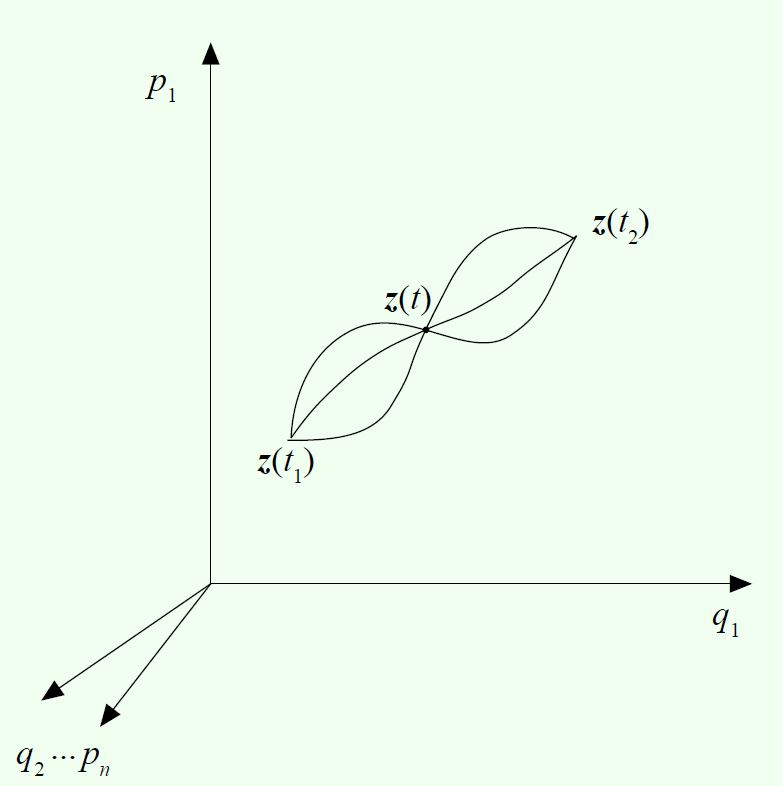
\includegraphics[width=0.500\linewidth]{1.jpg}
\caption{\textbf{Fig. 1} Phase-space variations of different paths.}\end{figure}

Replacing \(L\) by \(L_{ph}\) in \(S =
\int L dt\) we define the phase-space action integral
\begin{gather}
\begin{split}S_{ph}\left[q, p\right] = \int_{t_1}^{t_2}dt L_{ph}(q,p,\dot{q},t)=\int_{t_1}^{t_2}dt \left(p\cdot\dot{q}-H(q,p,t)\right)\end{split}\notag
\end{gather}
We know from variational calculus that \(S_{ph}\) is stationary under arbitrary
variations of the phase-space path (with endpoints fixed), explicitly, we get:
\begin{gather}
\begin{split}\delta S_{ph} =&\delta\int_{t_1}^{t_2}dt \left(p\cdot\dot{q}-H(q,p,t)\right) \\
=&\int_{t_1}^{t_2}dt \left(\delta p\cdot\dot{q}+p\cdot\delta\dot{q}-\delta p \frac{\partial H(q,p,t)}{\partial p}-\delta q \frac{\partial H(q,p,t)}{\partial q}\right) \\
=&p\delta q\left. \right |_{t_1}^{t_2}+\int_{t_1}^{t_2}dt \left\{\delta p\cdot\left[\dot{q}-\frac{\partial H(q,p,t)}{\partial p}\right]-\delta q\cdot\left[\dot{p}+ \frac{\partial H(q,p,t)}{\partial q}\right]\right\}\end{split}\notag
\end{gather}
which gives us the \textbf{Hamilton's equations}:
\begin{gather}
\begin{split}\dot{p}=-\frac{\partial H}{\partial q} \qquad \dot{q}=\frac{\partial H}{\partial p}\end{split}\notag
\end{gather}
\begin{notice}{note}{Note:}
More generally, the phase-space Lagrangian can depend on \(\dot{p}\) as well, and makes the Lagrange's equations become:
\begin{gather}
\begin{split}\frac{\delta L_{ph}(q,\dot{q},p,\dot{p})}{\delta q}=&\frac{\partial L_{ph}}{\partial q}-\frac{d}{dt}\frac{\partial L_{ph}}{\partial \dot{q}}=0 \\
\frac{\delta L_{ph}(q,\dot{q},p,\dot{p})}{\delta p}=&\frac{\partial L_{ph}}{\partial p}-\frac{d}{dt}\frac{\partial L_{ph}}{\partial \dot{p}}=0\end{split}\notag
\end{gather}\end{notice}

\textbf{References}
\begin{enumerate}
\item {}
L.D. Landau \& E.M. Lifshitz, \emph{Mechanics}.

\item {}
Lecture notes by \textbf{Bob Dewar} on website \href{http://people.physics.anu.edu.au/~rld105/C01\_ClassMech/}{Classical Mechanics}.

\end{enumerate}


\chapter{Topological Insulator:}
\label{index:topological-insulator}

\section{Lecture notes}
\label{TI/Lecture notes/main:lecture-notes}\label{TI/Lecture notes/main::doc}\label{TI/Lecture notes/main:id1}
Here is the lecture notes on TI, which is based on the lecture notes given by Janos Asboth, Laszlo Oroszlany, and Andras Palyi, \href{http://fizipedia.bme.hu/images/1/14/Topological\_insulators.pdf}{Here} is the resource, and you can also download a copy \href{https://github.com/bczhu/phyx/raw/master/\_static/files/TI.pdf}{here}.


\subsection{Lecture 1 : 1-d SSH model}
\label{TI/Lecture notes/1::doc}\label{TI/Lecture notes/1:lecture-1-1-d-ssh-model}

\subsubsection{The Su-Schrieffer--Heeger (SSH) model}
\label{TI/Lecture notes/1:the-su-schrieffer-heeger-ssh-model}
The simplest non-trivial topology : 1-d lattice.

Peierls instability makes the atoms dimerize.

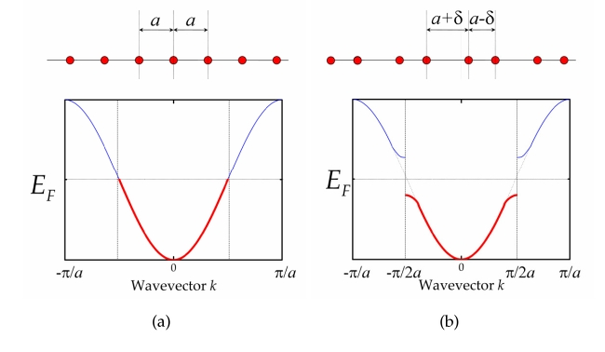
\includegraphics[width=0.5\textwidth]{11.png}

Polyacetylene Structure: 

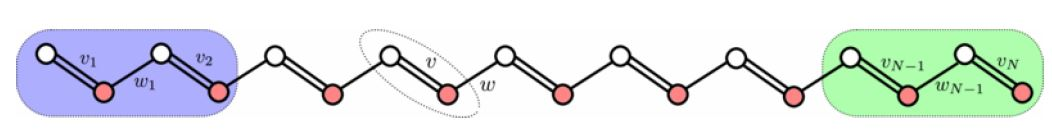
\includegraphics[width=0.5\textwidth]{2.jpg}


\subsubsection{Tight-binding method-first quantization}
\label{TI/Lecture notes/1:tight-binding-method-first-quantization}\begin{figure}[htbp]
\centering
\capstart

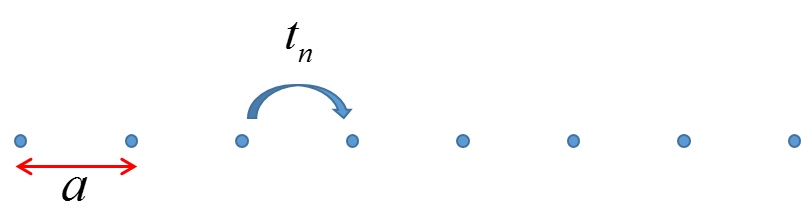
\includegraphics[width=0.5\textwidth]{31.png}
\caption{1-d atom chain}\end{figure}

Tight-binding method: Single electron total Hamiltonian in atom chain:
\begin{gather}
\begin{split}H=\frac{p^2}{2m}+U(x)\end{split}\notag
\end{gather}
with periodical potential: \(U(x+na)=U(x)\)

Assume single atom potential \(V(x)\) with Hamiltonian
\begin{gather}
\begin{split}H_0=\frac{p^2}{2m}+V(x)\end{split}\notag
\end{gather}

\bigskip\hrule{}\bigskip


and well solved eigen-value and eigen-wave-function:(consider only one
state)
\begin{gather}
\begin{split}H_0\phi(x)=E_0\phi(x)\end{split}\notag
\end{gather}
Do the combination
\begin{gather}
\begin{split}\psi(x)=\sum\limits_n a_n\phi_n\end{split}\notag
\end{gather}
with \(\phi_n=\phi(x-x_n), x_n=na\). Define
\(\Delta U(x)=U(x)-V(x)\), and substitute following equation
\begin{gather}
\begin{split}H\psi=\left(H_0+\Delta U\right)\psi=E\psi\end{split}\notag
\end{gather}
we get
\begin{gather}
\begin{split}\sum_n \langle \phi_m|\Delta U(x-x_n)|\phi_n\rangle a_n=(E-E_0)a_m\end{split}\notag
\end{gather}

\bigskip\hrule{}\bigskip


Define:
\(\langle \phi(x-ma+na)|\Delta U(x) |\phi(x)\rangle=-J(x_m-x_n)\)

We get:
\begin{gather}
\begin{split}-\sum_n J(x_m-x_n) a_n=(E-E_0) a_m\end{split}\notag
\end{gather}
Because of the Tranformation symmetry of the Hamiltonian, the resulting
wavefunction \(\psi(x)\) should take Bloch form, which means we
should have the solution \(a_m=e^{ikx_m}\), then, we get
\begin{gather}
\begin{split}E-E_0=-\sum_n J(x_n)e^{-ikx_n}\end{split}\notag
\end{gather}
Consider only the nearest-hopping interaction, define
\(J_0=J(0), J=J(\pm a)\), then we have:
\begin{gather}
\begin{split}E-E_0+J_0=&-J(e^{ika}+e^{-ika}) \\
=&-2Jcoska\end{split}\notag
\end{gather}

\subsubsection{Second quantization}
\label{TI/Lecture notes/1:second-quantization}
In the second quantization language, the expectation value of energy
becomes a operator, set \(\mathscr{H}=\frac{p^2}{2m}+U(x)\), we have
\begin{gather}
\begin{split}H=\langle \psi|\mathscr{H}|\psi \rangle \Rightarrow \hat{H}=\sum_{m,n}\hat{c}_m^\dagger H_{mn}\hat{c}_n\end{split}\notag
\end{gather}
with
\(\psi \to \hat{\psi}=\sum\limits_n \hat{c}_n \phi_n, H_{mn}=\langle \phi|\mathscr{H}|\phi \rangle\)
\(\phi_n\) is a orthonormal and complete basis in \emph{Hilbert space},
like plane-waves \(e^{ikx}\) or energy eigen-states of \(H_0\),
\(\mathscr{H}\) is the energy operator in single particle first
quantization picture, which can only act on Hilbert space, while the
second quantization energy operator \(\hat{H}\) acts on \emph{Fock
space}. Here, in tight-binding method, \(\phi_n\) is the
wave-function of site \(n\) of the energy eigen-state \(H_0\).


\bigskip\hrule{}\bigskip


Consider only the nearest interaction, we have:
\begin{gather}
\begin{split}\hat{H}=\sum_{n=1}^M \hat{c}_n^\dagger \hat{c}_{n+1}t_n+h.c.\end{split}\notag
\end{gather}
\(h.c.\) means hermitian conjugation. Rewrite it in matrix form:
\(\hat{H}=\sum\limits_{mn}\hat{c}_m \tilde{H}_{mn}c_n\), we have
\begin{gather}
\begin{split}\tilde{H}_{mn}=\begin{pmatrix} 0 & t_1 &0 & \cdots&t_M^*\\
t_1^* &0&t_2&\cdots&0\\
0&t_2^*&0&\cdots&0\\
\vdots&\vdots&\vdots&\vdots&\vdots\\
t_M&0&0&t_{M-1}^*&0
\end{pmatrix}\end{split}\notag
\end{gather}
In the case when \(t=t_n\), \(\hat{c}_n\) satisfy the Bloch
condition, we can transform it into momentum space, with
\(\hat{c}_n=\frac{1}{\sqrt{M}}\sum\limits_k \hat{c}_k e^{ikx_n}\),


\bigskip\hrule{}\bigskip


we can easily get
\begin{gather}
\begin{split}\hat{H}=\sum\limits_k \hat{c}_k^\dagger \hat{c}_k(te^{ika}+t^*e^{-ika})=\sum\limits_k \hat{c}_k^\dagger \hat{c}_k E(k)\end{split}\notag
\end{gather}
which gives us the dispersion relation:
\begin{gather}
\begin{split}E(k)=&te^{ika}+t^*e^{-ika}\\
=&2tcoska \qquad \textit{for t is real}\end{split}\notag
\end{gather}
On the other hand, keep in mind that we would get
\(c_n=e^{ik(n-1)a}c_1\), that is
\begin{gather}
\begin{split}\hat{H}=\begin{pmatrix}c_1^\dagger&c_2^\dagger&\cdots&c_M^\dagger \end{pmatrix}
\begin{pmatrix} 0 & t &0 & \cdots&t^*\\
t^* &0&t&\cdots&0\\
0&t^*&0&\cdots&0\\
\vdots&\vdots&\vdots&\vdots&\vdots\\
t&0&0&t^*&0
\end{pmatrix}
\begin{pmatrix}c_1\\c_2\\\vdots\\c_M\end{pmatrix}\end{split}\notag
\end{gather}

\bigskip\hrule{}\bigskip

\begin{gather}
\begin{split}\Rightarrow &\begin{pmatrix}c_1^\dagger&c_1^\dagger e^{-ika}&\cdots&c_1^\dagger e^{-ik(M-1)a} \end{pmatrix}
\begin{pmatrix} 0 & t &0 & \cdots&t^*\\
t^* &0&t&\cdots&0\\
0&t^*&0&\cdots&0\\
\vdots&\vdots&\vdots&\vdots&\vdots\\
t&0&0&t^*&0
\end{pmatrix}
\begin{pmatrix}c_1\\c_1 e^{ika}\\\vdots\\c_1e^{ik(M-1)a}\end{pmatrix}\\
=&\begin{pmatrix}c_1^\dagger&\cdots&c_1^\dagger \end{pmatrix}
\begin{pmatrix} te^{ika}+t^*e^{-ika} & 0&0\\
0&\ddots&0\\
0&0&te^{ika}+t^*e^{-ika}
\end{pmatrix}
\begin{pmatrix}c_1\\\vdots\\c_1\end{pmatrix}\end{split}\notag
\end{gather}
which also gives us \(E(k)=te^{ika}+t^*e^{-ika}\).


\bigskip\hrule{}\bigskip


More generally, \(t_n\) can be different from each other, for
example, if they are all different up to \(4\), but have a
super-periodicity with \(t_{5}=t_1\), then there will have 4
sub-bands, in the example we will consider below, we have two \(t\),
\(t_1\neq t_2\), and we have two sub-bands.

If each atom have a valance electron, then the above mentioned energy
band structure \(E(k)=2tcoska\) is not the stable fundamental mode,
it will dimerizes to lower the total energy, that means we'll get
following coupling case: 

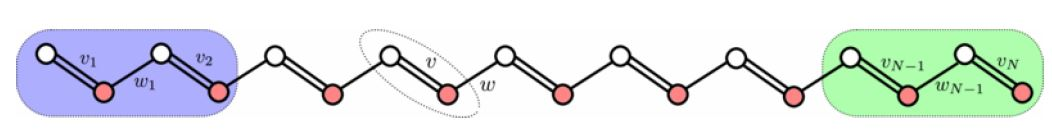
\includegraphics[width=0.5\textwidth]{2.jpg}

with the Hamiltonian:
\begin{gather}
\begin{split}H=\sum_{n=1}^N(v_n c_{n,1}^\dagger c_{n,2}+w_nc_{n,2}^\dagger c_{n+1,1}+h.c.)\end{split}\notag
\end{gather}
with \(M=2N\).


\subsubsection{Review}
\label{TI/Lecture notes/1:review}
In 1-d atom chain, we have got the Hamiltonian in second-quantization
frame as:
\begin{gather}
\begin{split}\hat{H}=\sum_{n=1}^M \hat{c}_n^\dagger \hat{c}_{n+1}t_n+h.c.\end{split}\notag
\end{gather}
\(h.c.\) means hermitian conjugation. Rewrite it in matrix form:
\(\hat{H}=\sum\limits_{mn}\hat{c}_m {H}_{mn}\hat{c}_n\), we have
\begin{gather}
\begin{split}\hat{H}=\begin{pmatrix}c_1^\dagger&c_2^\dagger&\cdots&c_M^\dagger \end{pmatrix}\begin{pmatrix} 0 & t_1 &0 & \cdots&t_M^*\\
t_1^* &0&t_2&\cdots&0\\
0&t_2^*&0&\cdots&0\\
\vdots&\vdots&\vdots&\vdots&\vdots\\
t_M&0&0&t_{M-1}^*&0
\end{pmatrix}\begin{pmatrix}c_1\\c_2\\\vdots\\c_M\end{pmatrix}\end{split}\notag
\end{gather}

\bigskip\hrule{}\bigskip

\begin{gather}
\begin{split}\hat{H}=\begin{pmatrix}c_1^\dagger&c_2^\dagger&\cdots&c_M^\dagger \end{pmatrix}\begin{pmatrix} 0 & t_1 &0 & \cdots&t_M^*\\
t_1^* &0&t_2&\cdots&0\\
0&t_2^*&0&\cdots&0\\
\vdots&\vdots&\vdots&\vdots&\vdots\\
t_M&0&0&t_{M-1}^*&0
\end{pmatrix}\begin{pmatrix}c_1\\c_2\\\vdots\\c_M\end{pmatrix}\end{split}\notag
\end{gather}
\(t_n\) can differ from each other.
\begin{enumerate}
\item {}
For a open chain with \(M\) atoms, we have \(t_M=0\), and
this matrix will give us \(M\) eigen-values and eigen-functions.

\item {}
Possess translational invariance with \(c_{n+1}=c_1e^{ikna}\), it
will be diagonalized with \(H(k)=te^{ika}+t^*e^{-ika}\).

\item {}
Staggered hopping parameters with \(t_1\neq t_2\), but have
property \(c_{2n+1}=c_1e^{iknb},c_{2n+2}=c_2e^{iknb}\). We can
block the Hamiltonian up in \(2\times 2\) blocks and also pair up
\(c_{2n+1},c_{2n+2}\).

\end{enumerate}


\bigskip\hrule{}\bigskip


The Hamiltonian:
\begin{gather}
\begin{split}H=\sum_{n=1}^N(v_n c_{n,1}^\dagger c_{n,2}+w_nc_{n,2}^\dagger c_{n+1,1}+h.c.)\end{split}\notag
\end{gather}
with \(M=2N\).
 
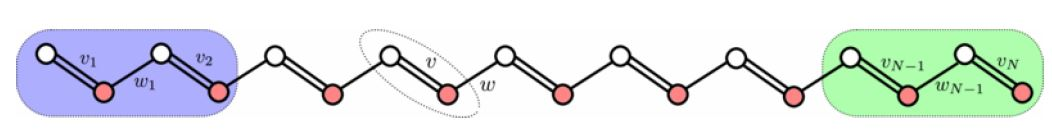
\includegraphics[width=0.5\textwidth]{2.jpg}

For a more beautiful notation, define
\(\mathbf{c}_n^\dagger=(c_{n,1}^\dagger,c_{n,2}^\dagger)=(c_{2n-1}^\dagger,c_{2n}^\dagger)\),
then we have
\begin{gather}
\begin{split}H=\sum_{m,n=1}^N \mathbf{c}_m^\dagger H_{mn}\mathbf{c}_n\end{split}\notag
\end{gather}
with
\begin{gather}
\begin{split}\mathbf{c}_n^\dagger H_{nn}\mathbf{c}_n=\begin{pmatrix}c_{n,1}^\dagger&c_{n,2}^\dagger\end{pmatrix}\begin{pmatrix}0&v_n\\v_n^*&0\end{pmatrix}\begin{pmatrix}c_{n,1}\\c_{n,2}\end{pmatrix}=\begin{pmatrix}c_{n,1}^\dagger&c_{n,2}^\dagger\end{pmatrix}U_n\begin{pmatrix}c_{n,1}\\c_{n,2}\end{pmatrix}\end{split}\notag
\end{gather}

\bigskip\hrule{}\bigskip


and
\begin{gather}
\begin{split}\mathbf{c}_n^\dagger H_{nn+1}\mathbf{c}_{n+1}=\begin{pmatrix}c_{n,1}^\dagger&c_{n,2}^\dagger\end{pmatrix}\begin{pmatrix}0&0\\w_n&0\end{pmatrix}\begin{pmatrix}c_{n+1,1}\\c_{n+1,2}\end{pmatrix}=\begin{pmatrix}c_{n,1}^\dagger&c_{n,2}^\dagger\end{pmatrix}T_n\begin{pmatrix}c_{n+1,1}\\c_{n+1,2}\end{pmatrix}\end{split}\notag
\end{gather}\begin{gather}
\begin{split}\mathbf{c}_{n+1}^\dagger H_{n+1n}\mathbf{c}_{n}=\begin{pmatrix}c_{n+1,1}^\dagger&c_{n+1,2}^\dagger\end{pmatrix}T_n^\dagger\begin{pmatrix}c_{n,1}\\c_{n,2}\end{pmatrix}\end{split}\notag
\end{gather}
when \(|m-n|>1\), we have \(H_{mn}=0\).

For example, for 6 cells (12 sites), we have
\begin{gather}
\begin{split}H=\begin{pmatrix}U_1&T_1&0&\cdots&T_6^\dagger\\
T_1^\dagger&U_2&T_2&\cdots&0\\
0&T_2^\dagger&U_3&\cdots&0\\
\vdots&\vdots&\vdots&\vdots&\vdots\\
T_6&0&0&\cdots&U_6
\end{pmatrix}\end{split}\notag
\end{gather}

\bigskip\hrule{}\bigskip

\begin{gather}
\begin{split}H_{mn}=\begin{pmatrix}U_1&T_1&0&\cdots&T_6^\dagger\\
T_1^\dagger&U_2&T_2&\cdots&0\\
0&T_2^\dagger&U_3&\cdots&0\\
\vdots&\vdots&\vdots&\vdots&\vdots\\
T_6&0&0&\cdots&U_6
\end{pmatrix}\end{split}\notag
\end{gather}\begin{itemize}
\item {}
Open chain: \(T_6=0\).

\item {}
Closed chain with translational symmetry, \(T_n=T,U_n=U\), with
\begin{gather}
\begin{split}U=\begin{pmatrix}0&v\\v^*&0\end{pmatrix},T=\begin{pmatrix}0&0\\w&0\end{pmatrix}\end{split}\notag
\end{gather}
Using three Pauli matrices
\begin{gather}
\begin{split}\sigma_x=\begin{pmatrix}0&1\\1&0\end{pmatrix},\sigma_y=\begin{pmatrix}0&-i\\i&0\end{pmatrix},\sigma_z=\begin{pmatrix}1&0\\0&-1\end{pmatrix}\end{split}\notag
\end{gather}
\end{itemize}


\bigskip\hrule{}\bigskip


We get
\begin{gather}
\begin{split}U=Re(v)\sigma_x-Im(v)\sigma_y,T=\frac{1}{2}w(\sigma_x-i\sigma_y)\end{split}\notag
\end{gather}
Using \(\mathbf{c}_n=e^{ik(n-1)b}\mathbf{c}_1\), we have
\begin{gather}
\begin{split}\hat{H}=\begin{pmatrix}\mathbf{c}_1^\dagger&\mathbf{c}_2^\dagger&\cdots&\mathbf{c}_N^\dagger \end{pmatrix}
\begin{pmatrix} U & T &0 & \cdots&T^\dagger\\
T^\dagger &U&T&\cdots&0\\
0&T^\dagger&U&\cdots&0\\
\vdots&\vdots&\vdots&\vdots&\vdots\\
T&0&0&T^\dagger&U
\end{pmatrix}
\begin{pmatrix}\mathbf{c}_1\\\mathbf{c}_2\\\vdots\\\mathbf{c}_N\end{pmatrix}\end{split}\notag
\end{gather}\begin{gather}
\begin{split}\Rightarrow \begin{pmatrix}\mathbf{c}_1^\dagger&\mathbf{c}_1^\dagger e^{-ikb}&\cdots&\mathbf{c}_1^\dagger e^{-ik(N-1)b} \end{pmatrix}
\begin{pmatrix} U & T &0 & \cdots&T^\dagger\\
T^\dagger &U&T&\cdots&0\\
0&T^\dagger&U&\cdots&0\\
\vdots&\vdots&\vdots&\vdots&\vdots\\
T&0&0&T^\dagger&U
\end{pmatrix}
\begin{pmatrix}\mathbf{c}_1\\\mathbf{c}_1 e^{ikb}\\\vdots\\\mathbf{c}_1e^{ik(N-1)b}\end{pmatrix}\end{split}\notag
\end{gather}

\bigskip\hrule{}\bigskip

\begin{gather}
\begin{split}=\begin{pmatrix}\mathbf{c}_1^\dagger&\cdots&\mathbf{c}_1^\dagger \end{pmatrix}
\begin{pmatrix} U+Te^{ikb}+T^\dagger e^{-ikb} & &\\
&\ddots&\\
&&U+Te^{ikb}+T^\dagger e^{-ikb}
\end{pmatrix}
\begin{pmatrix}\mathbf{c}_1\\\vdots\\\mathbf{c}_1\end{pmatrix}\end{split}\notag
\end{gather}
which gives us
\(H=H(k)\oplus H(k)\cdots \oplus H(k)=\oplus_{n=1}^N H(k)\) with
\begin{gather}
\begin{split}H(k)=U+Te^{ikb}+T^\dagger e^{-ikb}=\mathbf{h}(k)\cdot \mathbf{\sigma}\end{split}\notag
\end{gather}
with
\begin{gather}
\begin{split}h_x(k)=&Re(v)+|w|cos(kb+arg(w))\\
h_y(k)=&-Im(v)+|w|sin(kb+arg(w))\\
h_z(k)=&0\end{split}\notag
\end{gather}
with \(w=|w|e^{i arg(w)}\).


\bigskip\hrule{}\bigskip

\begin{gather}
\begin{split}H(k)=\mathbf{h}(k)\cdot \mathbf{\sigma}\end{split}\notag
\end{gather}
with

with eigen-energy
\begin{gather}
\begin{split}E(k)=|\mathbf(h)(k)=\pm \sqrt{h_x^2+h_y^2+h_z^2}=\pm \sqrt{|v|^2+|w|^2+2|v||w|cos(kb+arg(v)+arg(w))}\end{split}\notag
\end{gather}
and eigen-wavefunctions
\begin{gather}
\begin{split}|\pm\rangle=\begin{pmatrix}\pm e^{-i\phi(k)}\\
1\end{pmatrix}\end{split}\notag
\end{gather}
with \(tan\phi=h_y/h_x\).


\bigskip\hrule{}\bigskip


For example, set \(arg(v)=arg(w)=0\), we have 

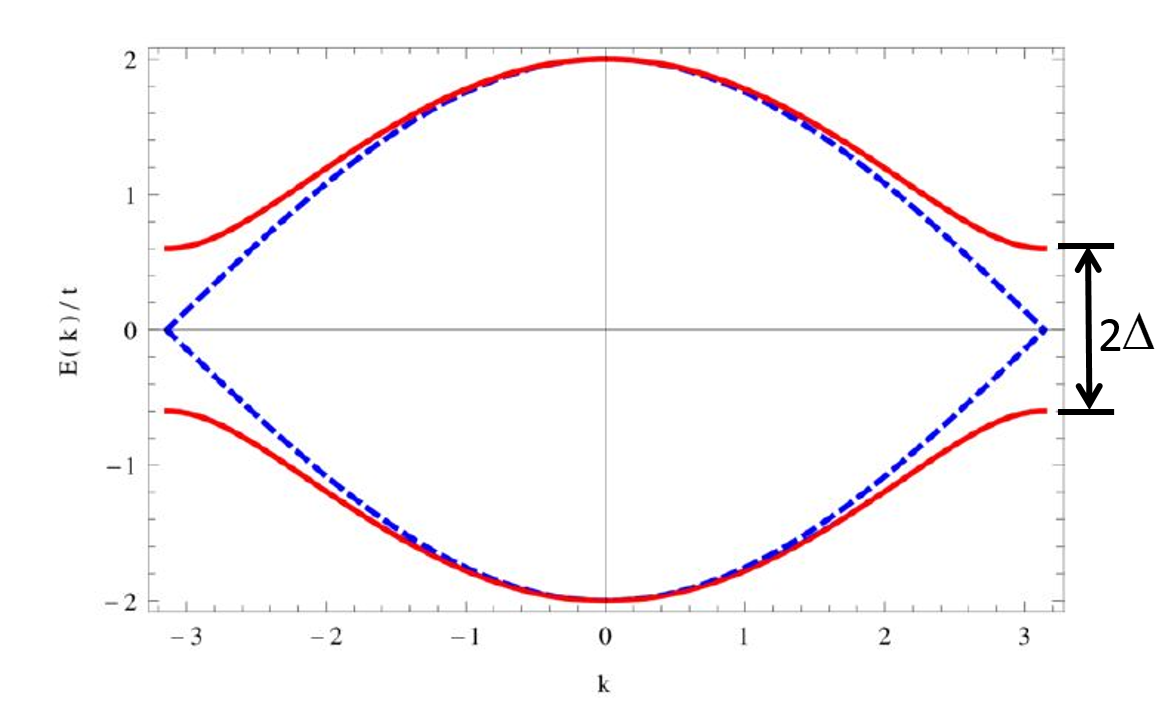
\includegraphics[width=0.5\textwidth]{energy.png}

Can nottell the difference \(|v|-|w|=\pm\delta\).


\bigskip\hrule{}\bigskip


Energy-band description is not completed, it can give us many
information, but not the whole, others are hidden in the wave-function.
Alternatively, recalling \(H(k)=\mathbf{h}(k)\cdot \mathbf{\sigma}\), the
Hamiltonian should contain the whole information, but we have only used
\(|h|\), in topological aspect, \(\mathbf{h}(k)\) will suffices.

Set \(arg(v)=0\),\(kb=[0,2\pi]\), we have two cases
\begin{itemize}
\item {}
\(|w|<|v|, \mathbf{inter}<\mathbf{intra}\)

\item {}
\(|w|>|v|, \mathbf{inter}>\mathbf{intra}\)

\end{itemize}


\bigskip\hrule{}\bigskip

\begin{figure}[htbp]
\centering
\capstart

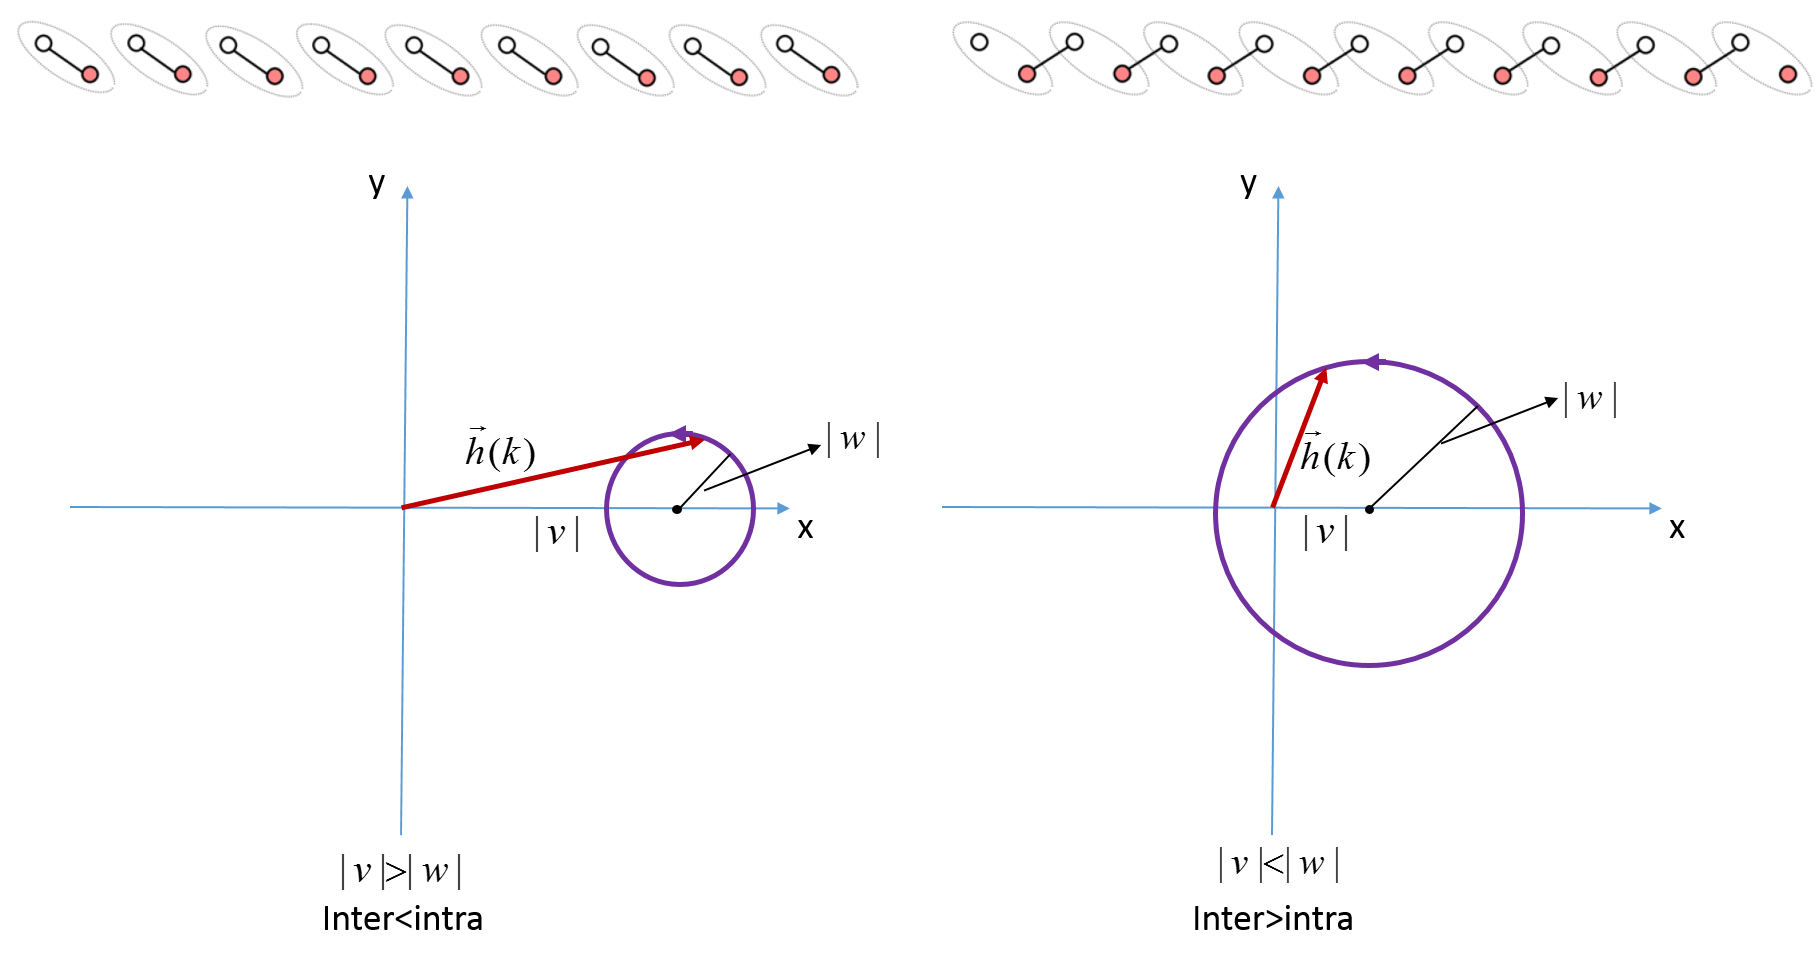
\includegraphics[width=0.8\textwidth]{two.png}
\caption{two cases}\end{figure}


\subsubsection{winding number}
\label{TI/Lecture notes/1:winding-number}
\(H(k)=\mathbf{h}(k)\cdot \mathbf{\sigma}\), \(\mathbf{h}(k)=0\) is a
degenerate point with \(|v|=|w|\), two bands cross, define
\(h(k)=h_x(k)+ih_y(k)\), we have
\begin{gather}
\begin{split}H(k)=\begin{pmatrix}0&h^*(k)\\h(k)&0\end{pmatrix}\end{split}\notag
\end{gather}\begin{gather}
\begin{split}ln(h)=ln(|h|)e^{iarg(h)}=ln(|h|)+iarg(h)\end{split}\notag
\end{gather}
define
\begin{gather}
\begin{split}\nu=\frac{1}{2\pi i}\int_{-\pi}^{\pi}dk\frac{d}{dk}ln(h(k))\end{split}\notag
\end{gather}
When
\begin{itemize}
\item {}
\(|w|>|v|, \nu=1, \mathbf{inter}>\mathbf{intra}\)

\item {}
\(|w|<|v|, \nu=0, \mathbf{inter}<\mathbf{intra}\)

\end{itemize}


\bigskip\hrule{}\bigskip


A example, \(N=20, M=2N=40, w=1, v=0.5\), we get eigen-energys:
\begin{figure}[htbp]
\centering
\capstart

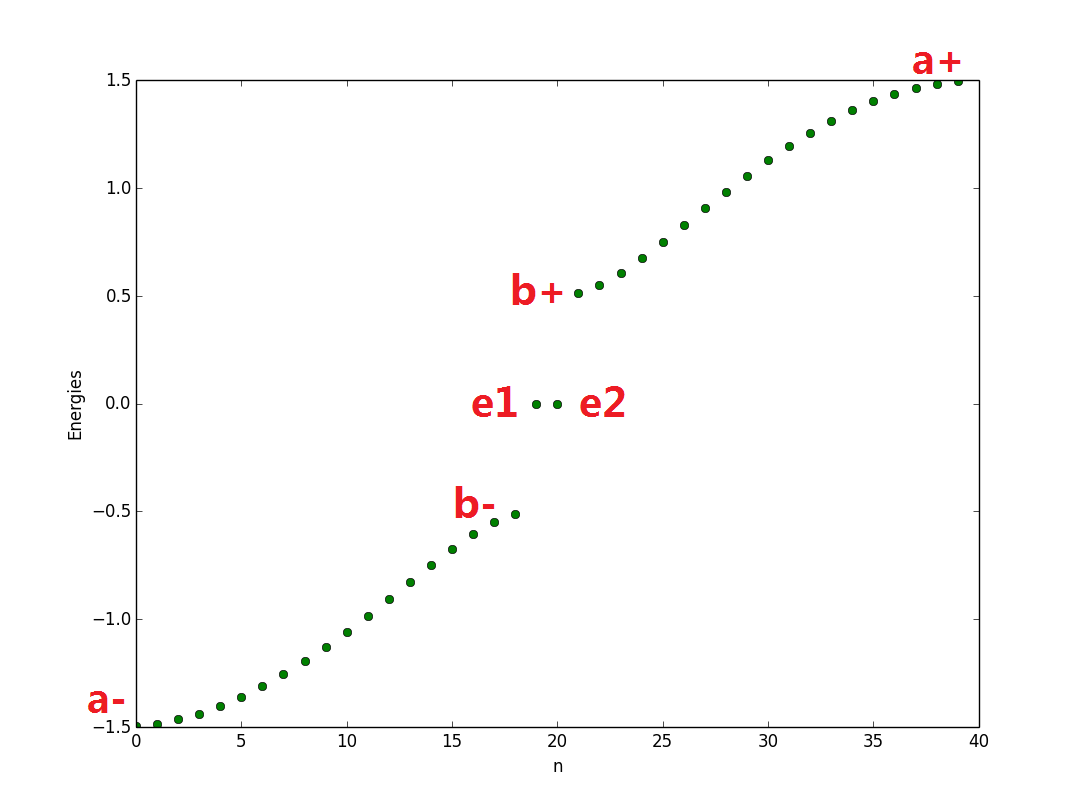
\includegraphics[width=0.5\textwidth]{4.png}
\caption{eigen-energy}\end{figure}


\bigskip\hrule{}\bigskip


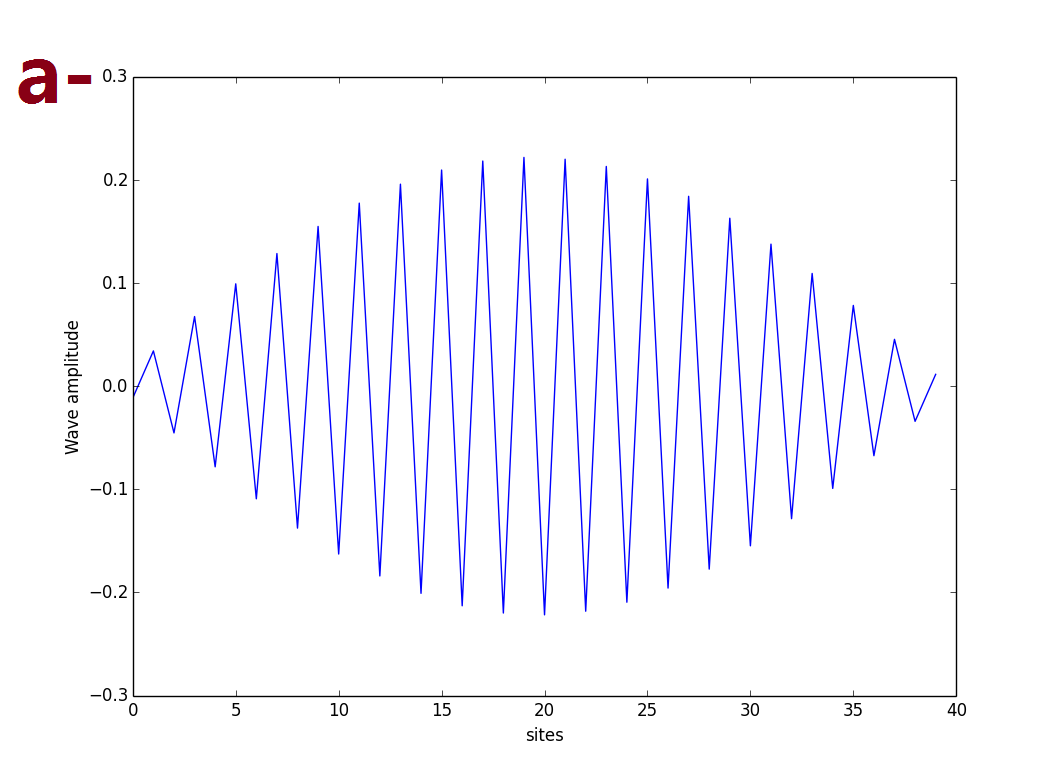
\includegraphics[width=0.5\textwidth]{a-.png} 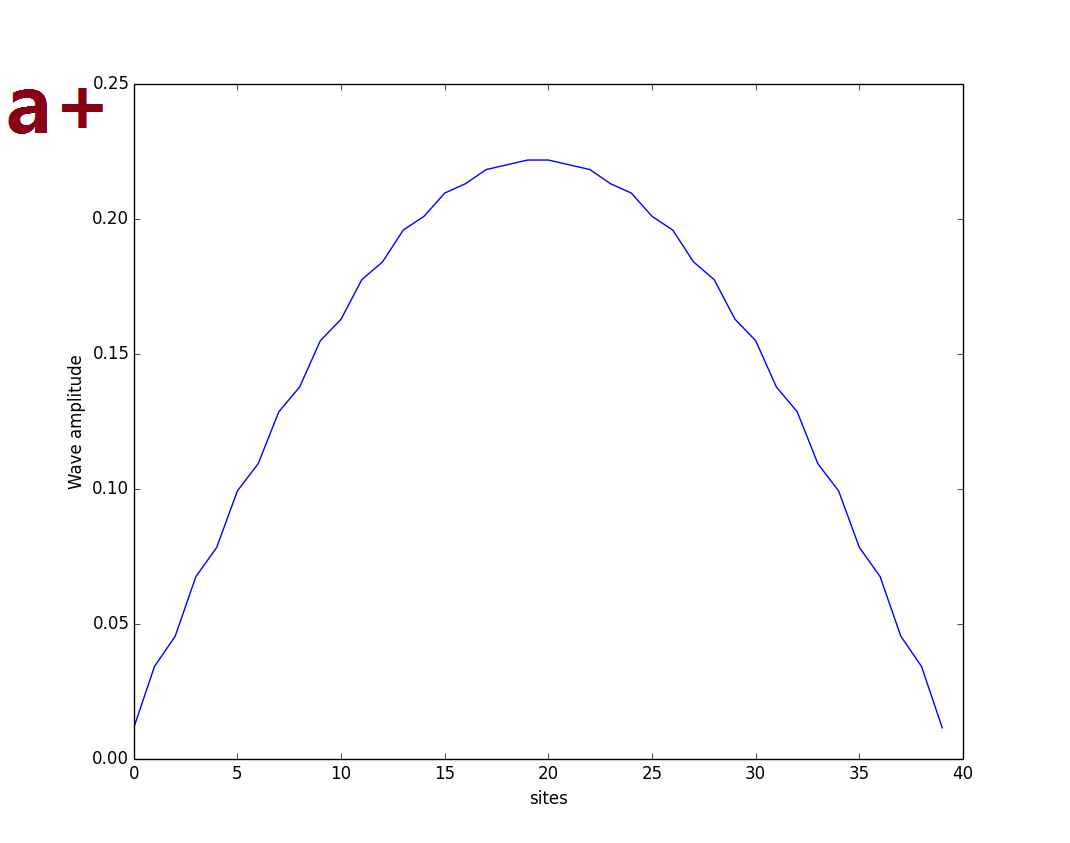
\includegraphics[width=0.5\textwidth]{a+.png}

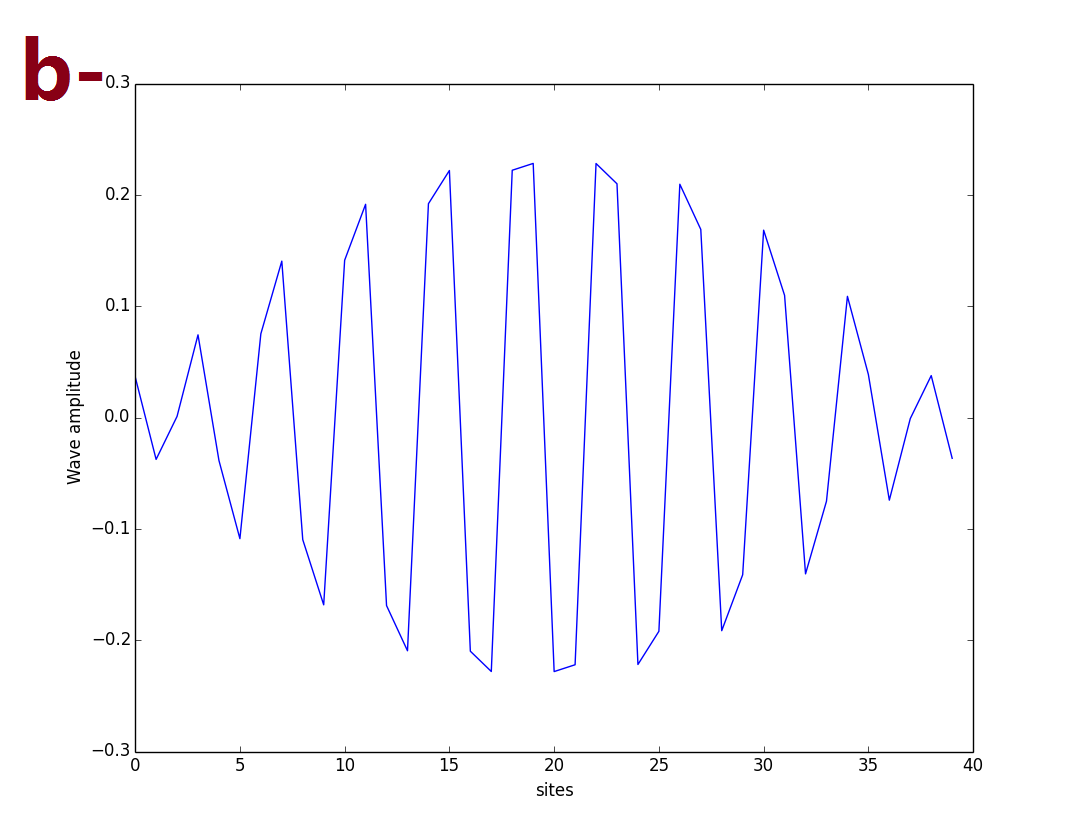
\includegraphics[width=0.5\textwidth]{b-.png} 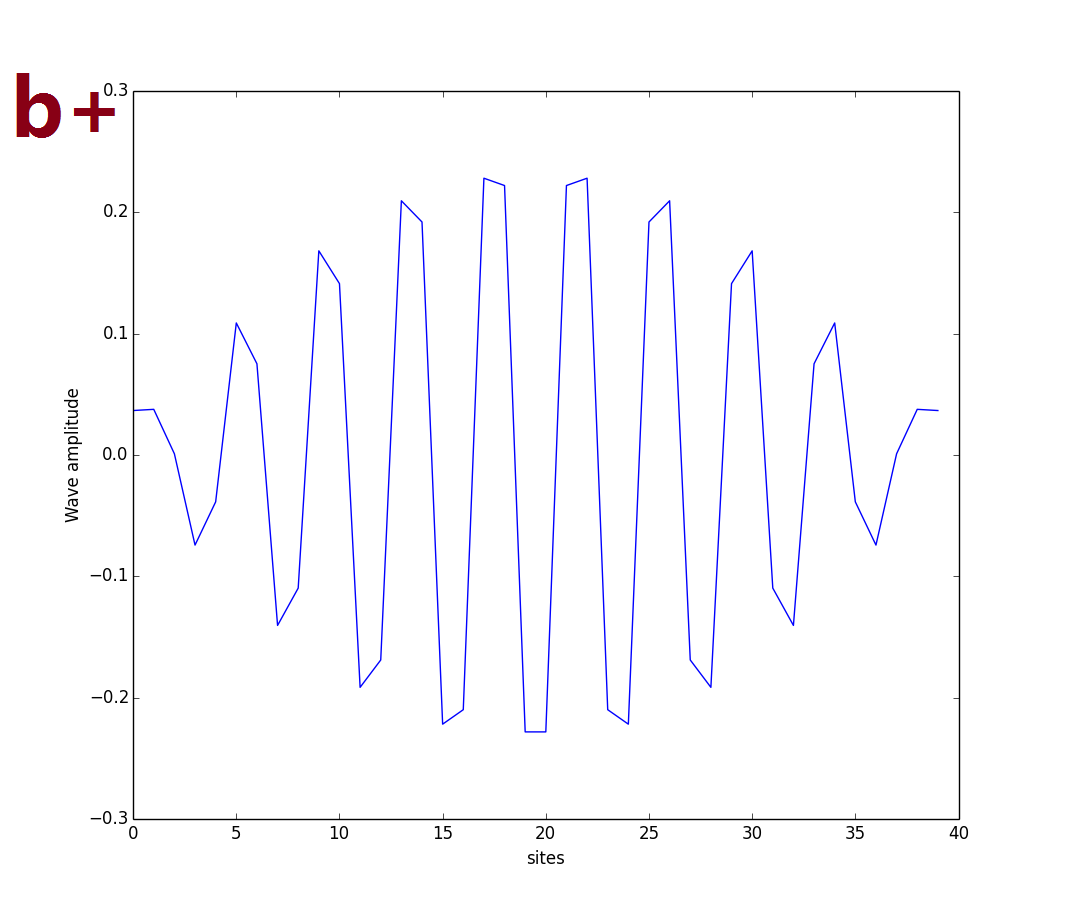
\includegraphics[width=0.5\textwidth]{b+.png}


\bigskip\hrule{}\bigskip


Edge-states: 

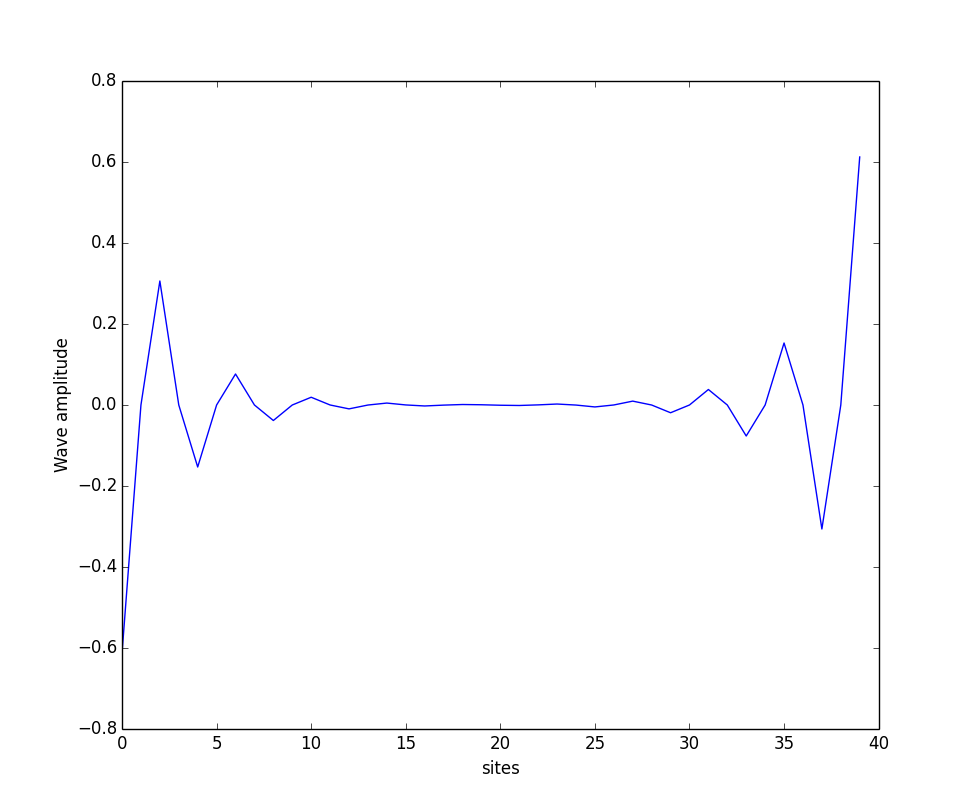
\includegraphics[width=0.5\textwidth]{c1.png} 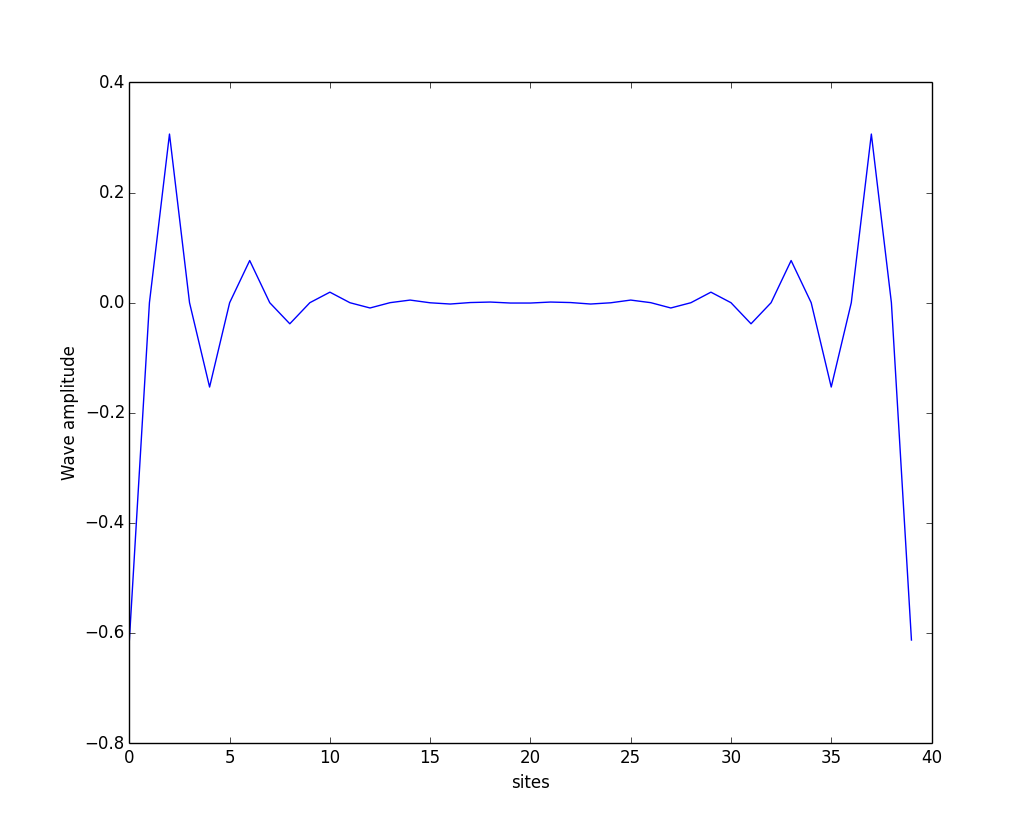
\includegraphics[width=0.5\textwidth]{c2.png}


\subsubsection{Chiral symmetry}
\label{TI/Lecture notes/1:chiral-symmetry}

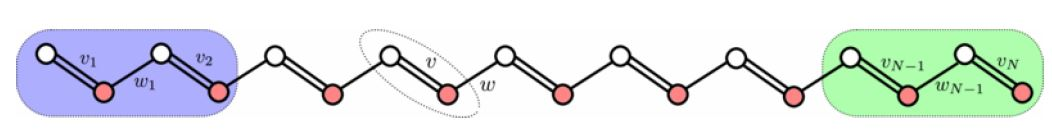
\includegraphics[width=0.5\textwidth]{2.jpg}

Recalling the Hamiltonian:
\begin{gather}
\begin{split}H=\sum_{n=1}^N(v_n c_{n,1}^\dagger c_{n,2}+w_nc_{n,2}^\dagger c_{n+1,1}+h.c.)\end{split}\notag
\end{gather}
Define projector operators:
\begin{gather}
\begin{split}P_A=\sum_n c_{n,1}^\dagger c_{n,1}, P_B=\sum_n c_{n,2}^\dagger c_{n,2}\end{split}\notag
\end{gather}
and the chiral operator \(\Sigma_z=P_A-P_B\), The matrix elements
of \(\Sigma_z\) vanish,
\(\langle 0|c_r \Sigma c^\dagger_s|0\rangle=0\) if sites \(r\)
and \(s\) are in different unit cells.


\bigskip\hrule{}\bigskip


In first-quantization, we have
\begin{gather}
\begin{split}H=\sum_{n=1}^N(v_n |n,1\rangle\langle n,2|+w_n|n,2\rangle\langle n+1,1|+h.c.)\end{split}\notag
\end{gather}
and
\begin{gather}
\begin{split}P_A=\sum_n |n,1\rangle\langle n,1|, P_B=\sum_n |n,2\rangle\langle n,2|\end{split}\notag
\end{gather}
In matrix form, we have
\begin{gather}
\begin{split}\Sigma_z=\sigma_z\oplus\sigma_z\oplus\cdots\oplus\sigma=\oplus_{n=1}^N \sigma_z\end{split}\notag
\end{gather}
\(\Sigma_z\) is \emph{local}, it does not mix site between unit cells,
and inherits the algebra from \(\sigma_z\):
\begin{gather}
\begin{split}\Sigma_z^\dagger\Sigma_z=1\end{split}\notag
\end{gather}\begin{gather}
\begin{split}\Sigma_z^2=1\end{split}\notag
\end{gather}

\bigskip\hrule{}\bigskip


Recalling
\begin{gather}
\begin{split}\begin{pmatrix} U_1 & T_1 &0 & \cdots&T_N^\dagger\\
T_1^\dagger &U_2&T_2&\cdots&0\\
0&T_2^\dagger&U_3&\cdots&0\\
\vdots&\vdots&\vdots&\vdots&\vdots\\
T_N&0&0&T_{N-1}^\dagger&U_N
\end{pmatrix}\end{split}\notag
\end{gather}
There are no \textbf{onsite terms} in the Hamiltonian, so we have
\begin{gather}
\begin{split}\Sigma_z H \Sigma_z=-H\end{split}\notag
\end{gather}
This is the chiral symmetry.

\begin{notice}{note}{Note:}
Actually, here, \(H\) is defined in momentum space, but
\(\Sigma_z\) in real space, we should write
\(\tilde{H}=U^\dagger H U\) for some unitary matrix \(U\), but
the property survives!
\end{notice}


\bigskip\hrule{}\bigskip


Consequences: For eigenstates \(|\psi_n\rangle\) of \(H\), we
have
\begin{gather}
\begin{split}H|\psi_n\rangle=E_n|\psi_n\rangle\end{split}\notag
\end{gather}\begin{gather}
\begin{split}H\Sigma_z|\psi_n\rangle=-\Sigma_zH|\psi_n\rangle=-\Sigma_zE_n|\psi_n\rangle=-E_n\Sigma_z|\psi_n\rangle\end{split}\notag
\end{gather}
If
\begin{itemize}
\item {}
\(E_n\neq 0\), two orthonormal states
\(|\psi_n\rangle, \Sigma_z|\psi_n\rangle\), which gives
\begin{gather}
\begin{split}\begin{pmatrix}\alpha^* &\beta^*\end{pmatrix}\begin{pmatrix}\alpha\\-\beta\end{pmatrix}=0\end{split}\notag
\end{gather}\begin{gather}
\begin{split}\Rightarrow |\alpha|^2=|\beta|^2\end{split}\notag
\end{gather}
\item {}
\(E_n=0\), \(\Sigma_z|\psi_n\rangle=\pm|\psi_n\rangle\),
gives \(|\psi_n\rangle=\begin{pmatrix}1 \\0\end{pmatrix}\) or
\(|\psi_n\rangle=\begin{pmatrix}0 \\1\end{pmatrix}\)

\end{itemize}


\bigskip\hrule{}\bigskip



\section{Berry's Phase}
\label{TI/Berry's Phase/main:id1}\label{TI/Berry's Phase/main::doc}\label{TI/Berry's Phase/main:berry-s-phase}

\subsection{Preliminary}
\label{TI/Berry's Phase/Preliminary:id1}\label{TI/Berry's Phase/Preliminary::doc}\label{TI/Berry's Phase/Preliminary:preliminary}

\subsection{some topics}
\label{TI/Berry's Phase/main:some-topics}\begin{itemize}
\item {}
fiber bundle

\item {}
gauge/parallel transport

\item {}
symmetry

\end{itemize}


\section{Weyl Semi-metal}
\label{TI/Weyl_semi-metal:id1}\label{TI/Weyl_semi-metal::doc}\label{TI/Weyl_semi-metal:weyl-semi-metal}

\subsection{Graphene}
\label{TI/Weyl_semi-metal:graphene}
In the tight-binding approximation, when only nearest neighborhood couplings are considered, the Hamiltonian of Graphene can be written as:
\begin{gather}
\begin{split}\hat{H}(\vec{k})=-t\begin{pmatrix}0 &h(\vec{k})\\h^*(\vec{k}) &0\end{pmatrix}\end{split}\notag
\end{gather}
where \(h(\vec{k})=\sum\limits_{\vec{\delta}_i}e^{i\vec{k}\cdot\vec{\delta}_i}=|h(\vec{k})|e^{i\phi(\vec{k})},\vec{\delta}_i\) are three position vectors shown in the following diagram.
\begin{figure}[htbp]
\centering
\capstart

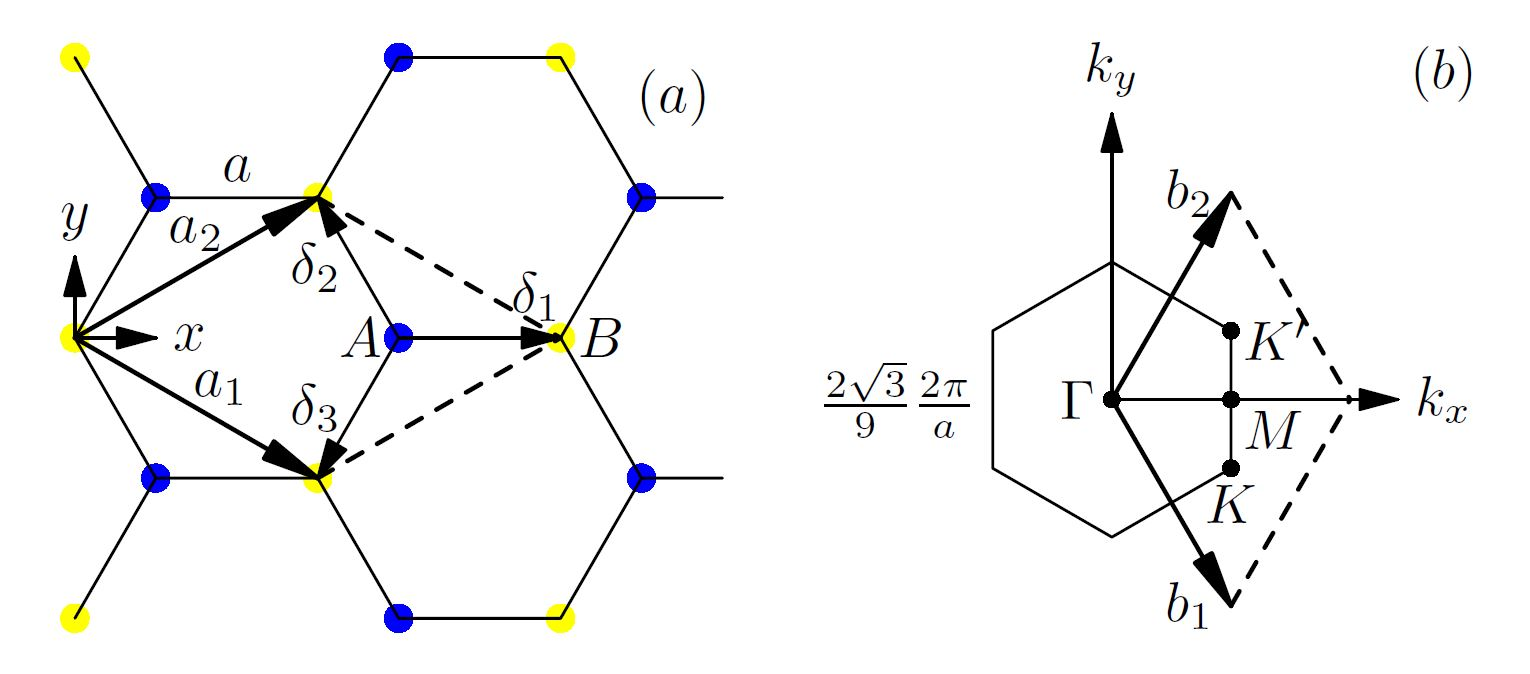
\includegraphics[width=0.700\linewidth]{1.png}
\caption{\textbf{Fig. 1}  Crystal Structure of Graphene: \(\vec{a}_{1}\) and \(\vec{a}_{2}\)
are Bravais crystal vectors for a Graphene unit cell. Each primitive
unit cell has two atomic sties, A and B. \(\vec{\delta}_{i}\) specifies
B-s' position around A site. (b) Brillouin Zone for Graphene
\(\vec{b}_{1}\) and \(\vec{b}_{2}\) are reciprocal vector basis for
intrinsic Graphene. Its corners are known as K and K' points.}\end{figure}

Then the Hamiltonian is:
\begin{gather}
\begin{split}\hat{H}(\vec{k})=-t|h(\vec{k})|\begin{pmatrix}0 &e^{i\phi(\vec{k})}\\e^{-i\phi(\vec{k})} &0\end{pmatrix}\end{split}\notag
\end{gather}
with the eigen-value: \(E(\vec{k})=-t|h(\vec{k})|\) and eigen-function (only show one of the two):
\begin{gather}
\begin{split}u(\vec{k})=\frac{1}{\sqrt{2}}\begin{pmatrix}e^{i\phi(\vec{k})/2}\\e^{-i\phi(\vec{k})/2} \end{pmatrix}e^{i\psi(\vec{k})}\end{split}\notag
\end{gather}
We should notice that the \(1/2\) factor is quite important here, when \(\phi\) changes \(2\pi\), the wave-function does not return to its original value, but with a minus sign. If instead, we want the wave-function to be single valued, the function :math:{\color{red}\bfseries{}{}`}psi(vec\{k\}){}`should change accordingly.

At the vicinity of Dirac point (K or K', here we expand the things near K), we have:
\begin{gather}
\begin{split}\hat{H}(\vec{K}+\vec{q})=&\alpha\begin{pmatrix}0&q_x+iq_y\\q_x-iq_y&0\end{pmatrix}=\alpha(q_x\sigma_x-q_y\sigma_y) \\
=&\alpha|q|\begin{pmatrix}0 &e^{i\phi(\vec{q})}\\e^{-i\phi(\vec{q})} &0\end{pmatrix}\end{split}\notag
\end{gather}
We can see that the general \(\phi\) turn out to be the angle of \(\vec{q}\) with the x axis. Then, wind a circle around the Dirac point K at some energy in the band structure shown below (Fig. 2(a)), the corresponding \(\phi\) (Fig. 2(c))winds one round too.
\begin{figure}[htbp]
\centering
\capstart

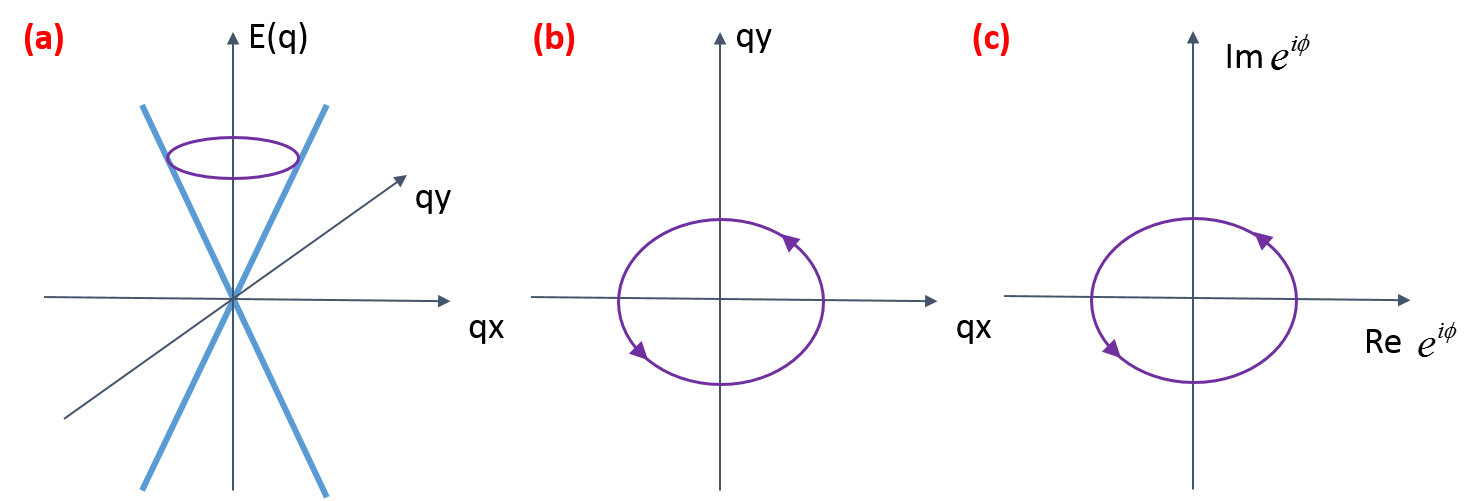
\includegraphics[width=0.750\linewidth]{2.png}
\caption{\textbf{Fig. 2} Dirac cone and the winding of \(\vec{q}\) and \(\phi\)}\end{figure}

So, if \(\vec{q}\) circles around the Dirac point one turn, \(\phi\) changes from 0 to \(2\pi\), in order to keep the basic wave-function \(u(\vec{q})\) single-valued, \(\psi\) \textbf{must} changes \(\pi\).

More explicitly, we calculate the vector potential in momentum space with:
\begin{gather}
\begin{split}\vec{A}(\vec{k})=i\langle u^\dagger |\nabla_{\vec{k}} u(\vec{k})\rangle=-\nabla \psi(\vec{k})\end{split}\notag
\end{gather}
Then we get:
\begin{gather}
\begin{split}\gamma=\oint{\vec{A}\cdot d\vec{k}} =-\psi(\phi=2\pi)+\psi(\phi(0))=-\pi\end{split}\notag
\end{gather}
We got the Berry's phase \(\gamma=\pm\pi\). It is this non-trivial phase of the equal-frequency surface that makes us call it \textbf{Weyl semi-metal}, and the \emph{Dirac points} called \emph{Weyl nodes}.


\subsection{Three dimension: Weyl semi-metal and Chern number}
\label{TI/Weyl_semi-metal:three-dimension-weyl-semi-metal-and-chern-number}
In three dimension, things can goes the same way. Using a simple model with Hamiltonian:
\begin{gather}
\begin{split}H(\vec{k})=\left[-2t_x\left(cosk_x-cosk_0\right)+m\left(2-cosk_y-cosk_z\right)\right]\sigma_x+2t_ysink_y\sigma_y+2t_zsink_z\sigma_z\end{split}\notag
\end{gather}
It has two Weyl nodes: \(\vec{K}=\pm\left(k_0,0,0\right)\), which means if we treat \(k_x\) as a variable, only when \(k_x=\pm k_0\), the corresponding energy band \(E_{k_x}(k_y,k_z)\) is crossing at the point \(k_y,k_z=(0,0)\).

Also, at the Weyl node (say \(k_x=k_0\)), we have:
\begin{gather}
\begin{split}H(\vec{K}+\vec{q})=v_xq_x\sigma_x+v_yq_y\sigma_y+v_zq_z\sigma_z\end{split}\notag
\end{gather}
with \(v_x=2t_xsink_0,v_y=2t_y,v_z=2t_z\). Without loss of generality, we can set \(v_x=v_y=v_z\) (the only effect is the shape changing from sphere to ellipsoid, which has no effect on the topology), then we get:
\begin{gather}
\begin{split}H(\vec{K}+\vec{q})=v\vec{q}\cdot\vec{\sigma}\end{split}\notag
\end{gather}
with eigen-value: \(E(\vec{k})=v|\vec{q}|\) and eigen-function (only show one of the two):
\begin{gather}
\begin{split}u(\vec{k})=\begin{pmatrix}sin\frac{\theta}{2}\\-cos\frac{\theta}{2}e^{i\phi}\end{pmatrix}e^{i\chi}\end{split}\notag
\end{gather}
It is easy to find that this wave-function will give us a magnetic field with a monopole at \(\vec{K}\), which will give us non-trivial equal-frequency surface Chern number \(C=1\).


\subsection{Bulk-boundary corresponding}
\label{TI/Weyl_semi-metal:bulk-boundary-corresponding}
In order to see things clearer, also, to see the connection of Weyl semi-metal with Topological insulator, we treat \(k_x\) as a variable, the Hamiltonian is:
\begin{gather}
\begin{split}H_{k_x}(k_y,k_z)=\vec{h}(\vec{k})\cdot\sigma=\left[-2t_x\left(cosk_x-cosk_0\right)+m\left(2-cosk_y-cosk_z\right)\right]\sigma_x+2t_ysink_y\sigma_y+2t_zsink_z\sigma_z\end{split}\notag
\end{gather}
For example, we set \(t_x=t_y=t_z=1,m=2,k_0=1\), three typical energy band dispersions shown below:
\begin{figure}[htbp]
\centering
\capstart

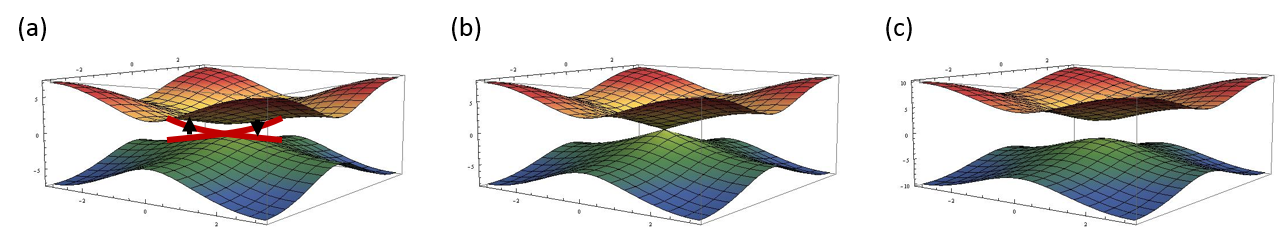
\includegraphics[width=0.800\linewidth]{3.png}
\caption{\textbf{Fig. 3} Typical energy band dispersion with (a) \(k_x=0\), (b) \(k_x=k_0=1\), (c) \(k_x=2\).}\end{figure}

To see if the system with \(k_x\neq k_0\) is a topological insulator or not, we can plot the diagram of \(\vec{h}(k_y,k_z)\), and see how many times the resulting torus incorporates the origin point. Typical shape of the torus shows below:
\begin{figure}[htbp]
\centering
\capstart

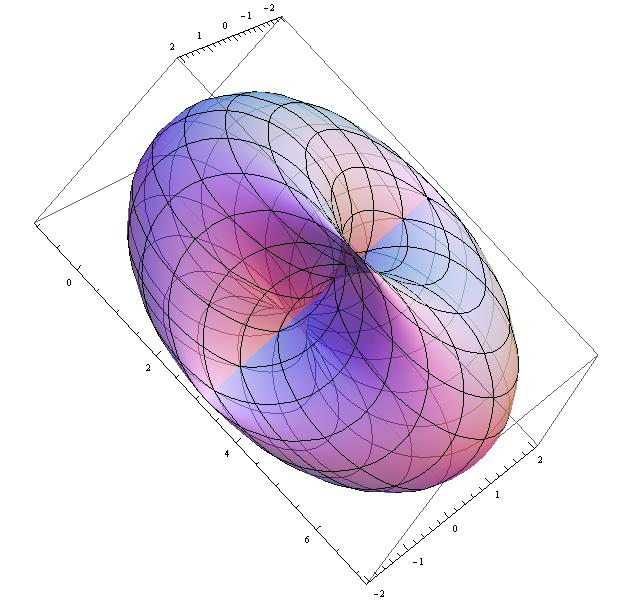
\includegraphics[width=0.450\linewidth]{4.jpg}
\caption{\textbf{Fig. 4} Typical torus of \(\vec{h}(k_y,k_z)\) with \(k_x=0\).}\end{figure}

We found that at the region \(k_x=[-k_0,k_0]\), the origin point is in the torus once with Chern number \(C=1\), outside of that, we got \(C=1\) (Noticing we have \(k_x=[-\pi,\pi]\)) . This is why we plot the edge state in Fig. 4(a), but not in Fig. 4(c). In the non-trivial case, for any energy inside the gap, we get a edge state, so different \(k_x\) will give us a edge-state line, which is called \emph{Fermi-arc}, especially, when we look at the case of Fermi surface with energy \(E=0\), the Fermi-arc stretch from one Weyl node to another, like the picture shown below:
\begin{figure}[htbp]
\centering
\capstart

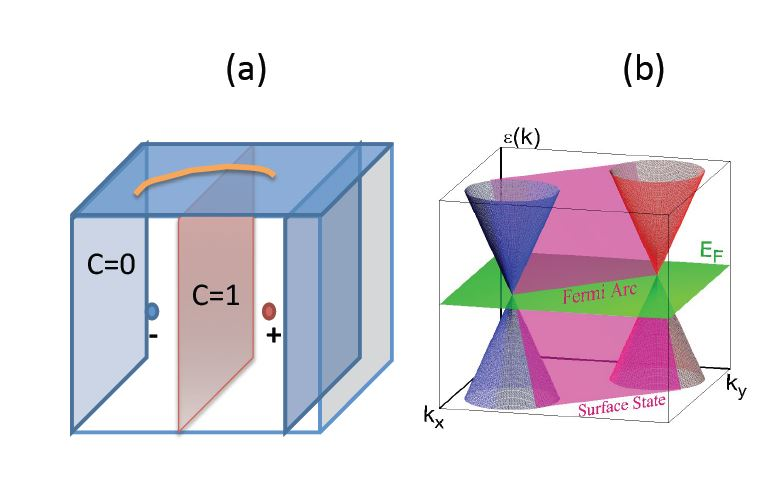
\includegraphics[width=0.600\linewidth]{5.png}
\caption{\textbf{Fig. 5} Fermi arc.}\end{figure}

Alternatively, we can look at the Bulk-boundary corresponding another way. The Weyl points behave like “magnetic” monopoles in momentum space whose charge is given by the chirality; they are actually a source of “Berry flux” rather than magnetic flux.

Consider a curve in the surface Brillouin zone encircling the projection of the bulk Weyl point, which is traversed counterclockwise as we vary the parameter \(\lambda: 0 \to 2\pi; \mathbf{k}_{\lambda} = [k_x (\lambda),k_y (\lambda)]\) {[}see Fig. 6(a){]}.We show that the energy \(\lambda\) of a surface state at momentum \(\mathbf{k}_{\lambda}\) crosses \(E = 0\) at some value of \(\lambda\). Consider \(H(\lambda,k_z) = H(\mathbf{k}_{\lambda},k_z)\), which can be interpreted as the gapped Hamiltonian of a two-dimensional system (with \(\lambda\) and \(k_z\) as the two momenta). The two periodic parameters \(\lambda\) , \(k_z\) define the surface of a torus in momentum space. The Chern number of this two-dimensional band structure is given by the Berry curvature integration: \(\frac{1}{2\pi}\int\mathscr{F}dk_zd\lambda\), which, by the Stokes theorem, simply corresponds to the net monopole density enclosed within the torus. This is obtained by summing the chiralities of the enclosed Weyl nodes. Consider the case when the net chirality is unity, corresponding to a single enclosed Dirac node. Then, the two-dimensional subsystem is a quantum Hall insulator with unit Chern number. When the
system is given a boundary at \(z = 0\), we expect a chiral edge state for this subsystem {[}see Fig. 6(b){]}. Hence, this surface state crosses zero energy somewhere on the surface Brillouin zone \(\mathbf{k}_{\lambda_0}\) . Such a state can be obtained for every curve enclosing the Weyl point. Thus, at zero energy, there is a Fermi line in the surface Brillouin zone, that terminates at the Weyl point momenta {[}see Fig. 6(c){]}. An arc beginning on a Weyl point of chirality c has to terminate on a Weyl point of the opposite chirality. Clearly, the net chirality of the Weyl points within the \((\lambda,k_z)\) torus was a key input in determining the number of these states. If Weyl points of opposite chirality line up along
the \(k_z\) direction, then there is a cancellation and no surface states are expected.
\begin{figure}[htbp]
\centering
\capstart

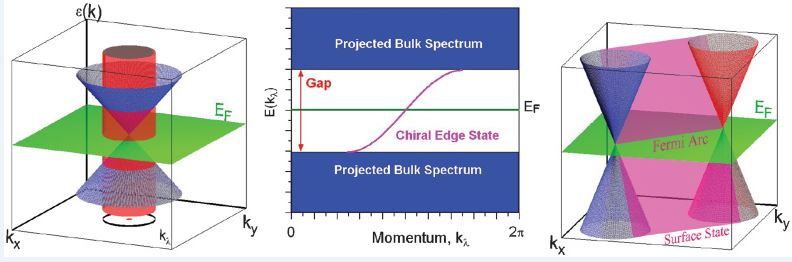
\includegraphics[width=0.700\linewidth]{6.png}
\caption{\textbf{Fig. 6} Illustration of surface states arising from bulk Weyl points.}\end{figure}

\textbf{References:}
\begin{enumerate}
\item {} \begin{enumerate}
\setcounter{enumi}{23}
\item {}
Wan, A.M. Turner, A. Vishwanath, and S.Y. Savrasov, Physical Review B \textbf{83}, 205101 (2011).

\end{enumerate}

\item {}
A.M. Turner, A. Vishwanath, and C.O. Head, Topological Insulators \textbf{6}, 293 (2013).

\item {} \begin{enumerate}
\setcounter{enumi}{5}
\item {}
Haldane, Physical Review Letters \textbf{93}, 206602 (2004).

\end{enumerate}

\end{enumerate}


\chapter{Condensed Matter Physics:}
\label{index:condensed-matter-physics}

\section{Linear response theory}
\label{CMP/linear response theory/main:id1}\label{CMP/linear response theory/main::doc}\label{CMP/linear response theory/main:linear-response-theory}

\subsection{Kubo formula}
\label{CMP/linear response theory/Kubo_formula:kubo-formula}\label{CMP/linear response theory/Kubo_formula::doc}\label{CMP/linear response theory/Kubo_formula:id1}
Many times, the world shows us as a \textbf{black box}, we can only get limited knowledge about it and the rest are filled with our \emph{theories}, in this way, theories can always changing and are never completed. we always use a probe to probe a system and check its response to this probe, and naturally, we expect when the perturbation of the probe is ignorable to the system, the response should be linear to the probe, which is called \textbf{linear response theory}. The most important result of linear response theory is consummated by \emph{Kubo formula}, we are now going to derive it.


\subsubsection{Zero temperature}
\label{CMP/linear response theory/Kubo_formula:id2}\label{CMP/linear response theory/Kubo_formula:zero-temperature}
Let \(\hat{H}_0\) be the full many-body Hamiltonian for some isolated system that we are interested in, and assume the existence of a set of eigenkets \(\{|n\rangle\}\) that diagonalize \(\hat{H}_0\) with associated
eigenvalues (energies) \(\varepsilon_n\).

In addition to \(\hat{H}_0\), we now turn on an external probe potential \(\hat{V}(t)\), such that the total Hamiltonian \(\hat{H}(t)\) satisfies:
\begin{gather}
\begin{split}\hat{H}(t)=\hat{H}_0+e^{\eta t}\hat{V}(t)\end{split}\notag
\end{gather}
\begin{notice}{note}{Note:}
The additional factor \(e^{\eta t}\) means we switch on the external potential adiabatically from \(t\to -\infty\), we'll see later that it is this factor gives us the way to detour the \emph{singular points}, it is an \emph{analytical continuation} which is a reflection of \emph{causality}.
\end{notice}

The Schr\"{o}dinger equation of the system now reads:
\begin{gather}
\begin{split}i\hbar\frac{\partial}{\partial t}|\psi(t)\rangle=(\hat{H}_0+e^{\eta t}\hat{V}(t))|\psi(t)\rangle\end{split}\notag
\end{gather}
\begin{notice}{warning}{Warning:}
us the way to detour the singular points, it is an analytical continuation which is a reflection of causality.
\end{notice}

\begin{notice}{important}{Important:}
us the way to detour the singular points, it is an analytical continuation which is a reflection of causality.
\end{notice}

\begin{notice}{hint}{Hint:}
us the way to detour the singular points, it is an analytical continuation which is a reflection of causality.
\end{notice}


\section{Fermi's Golden rule}
\label{CMP/Fermi's_Golden_rule:id1}\label{CMP/Fermi's_Golden_rule::doc}\label{CMP/Fermi's_Golden_rule:fermi-s-golden-rule}

\chapter{Some topics want to explore}
\label{index:some-topics-want-to-explore}\begin{itemize}
\item {}
Green's Function

\item {}
Dirac,Majorana,Weyl fermions

\end{itemize}


\chapter{Something about Python}
\label{index:something-about-python}

\section{Python 学习}
\label{Python/note:python}\label{Python/note::doc}\label{Python/note:id1}\begin{enumerate}
\item {}
\textbf{数组初始化}

\end{enumerate}

\begin{Verbatim}[commandchars=\\\{\}]
\PYG{c}{\PYGZsh{}初始化一维数组}
\PYG{n}{p1}\PYG{o}{=}\PYG{p}{[}\PYG{l+m+mi}{1}\PYG{p}{]}\PYG{o}{*}\PYG{l+m+mi}{100}

\PYG{c}{\PYGZsh{}初始化二维数组100*10}
\PYG{n}{p2}\PYG{o}{=}\PYG{p}{[}\PYG{p}{[}\PYG{l+m+mi}{1}\PYG{p}{]} \PYG{o}{*} \PYG{l+m+mi}{100} \PYG{k}{for} \PYG{n}{i} \PYG{o+ow}{in} \PYG{n+nb}{xrange}\PYG{p}{(}\PYG{l+m+mi}{10}\PYG{p}{)}\PYG{p}{]}
\PYG{c}{\PYGZsh{}Below does not work!}
\PYG{n}{p2}\PYG{o}{=}\PYG{p}{[}\PYG{p}{[}\PYG{l+m+mi}{1}\PYG{p}{]} \PYG{o}{*} \PYG{l+m+mi}{100}\PYG{p}{]}\PYG{o}{*}\PYG{l+m+mi}{10}
\PYG{c}{\PYGZsh{}Or we can use:}
\PYG{n}{p2}\PYG{o}{=}\PYG{p}{[}\PYG{p}{[}\PYG{n+nb+bp}{None} \PYG{k}{for} \PYG{n}{col} \PYG{o+ow}{in} \PYG{n+nb}{range}\PYG{p}{(}\PYG{l+m+mi}{100}\PYG{p}{)}\PYG{p}{]} \PYG{k}{for} \PYG{n}{row} \PYG{o+ow}{in} \PYG{n+nb}{range}\PYG{p}{(}\PYG{l+m+mi}{10}\PYG{p}{)}\PYG{p}{]}

\PYG{c}{\PYGZsh{}初始化三维维数组2*3*4}
\PYG{n}{p3}\PYG{o}{=}\PYG{p}{[}\PYG{p}{[}\PYG{p}{[}\PYG{l+m+mi}{1}\PYG{p}{]} \PYG{o}{*} \PYG{l+m+mi}{2} \PYG{k}{for} \PYG{n}{i} \PYG{o+ow}{in} \PYG{n+nb}{xrange}\PYG{p}{(}\PYG{l+m+mi}{3}\PYG{p}{)}\PYG{p}{]} \PYG{k}{for} \PYG{n}{j} \PYG{o+ow}{in} \PYG{n+nb}{xrange}\PYG{p}{(}\PYG{l+m+mi}{4}\PYG{p}{)}\PYG{p}{]}
\PYG{c}{\PYGZsh{}Or}
\PYG{n}{p3}\PYG{o}{=}\PYG{p}{[}\PYG{p}{[}\PYG{p}{[}\PYG{l+m+mi}{1} \PYG{k}{for} \PYG{n}{i} \PYG{o+ow}{in} \PYG{n+nb}{xrange}\PYG{p}{(}\PYG{l+m+mi}{2}\PYG{p}{)}\PYG{p}{]} \PYG{k}{for} \PYG{n}{j} \PYG{o+ow}{in} \PYG{n+nb}{xrange}\PYG{p}{(}\PYG{l+m+mi}{3}\PYG{p}{)}\PYG{p}{]} \PYG{k}{for} \PYG{n}{k} \PYG{o+ow}{in} \PYG{n+nb}{xrange}\PYG{p}{(}\PYG{l+m+mi}{4}\PYG{p}{)}\PYG{p}{]}
\PYG{c}{\PYGZsh{}Or}
\PYG{n}{p3}\PYG{o}{=}\PYG{p}{[}\PYG{p}{]}
\PYG{k}{for} \PYG{n}{i} \PYG{o+ow}{in} \PYG{n+nb}{range}\PYG{p}{(}\PYG{l+m+mi}{2}\PYG{p}{)}\PYG{p}{:}
    \PYG{n}{p3}\PYG{o}{.}\PYG{n}{append}\PYG{p}{(}\PYG{p}{[}\PYG{p}{]}\PYG{p}{)}
    \PYG{k}{for} \PYG{n}{j} \PYG{o+ow}{in} \PYG{n+nb}{range}\PYG{p}{(}\PYG{l+m+mi}{3}\PYG{p}{)}\PYG{p}{:}
        \PYG{n}{p3}\PYG{p}{[}\PYG{n}{i}\PYG{p}{]}\PYG{o}{.}\PYG{n}{append}\PYG{p}{(}\PYG{p}{[}\PYG{p}{]}\PYG{p}{)}
        \PYG{k}{for} \PYG{n}{k} \PYG{o+ow}{in} \PYG{n+nb}{range}\PYG{p}{(}\PYG{l+m+mi}{4}\PYG{p}{)}\PYG{p}{:}
            \PYG{n}{p3}\PYG{p}{[}\PYG{n}{i}\PYG{p}{]}\PYG{p}{[}\PYG{n}{j}\PYG{p}{]}\PYG{o}{.}\PYG{n}{append}\PYG{p}{(}\PYG{l+m+mi}{0}\PYG{p}{)}
\end{Verbatim}
\begin{enumerate}
\item {}
python 中的内积 \code{dot} 是没有复共轭的,\code{vdot} 有,而matlab \code{dot(a,b)} 是对a取复共轭的。

\end{enumerate}


\bigskip\hrule{}\bigskip

\begin{figure}[htbp]
\centering
\href{http://creativecommons.org/licenses/by-nc-sa/3.0/us/}{
\includegraphics{cc_byncsa.png}}\end{figure}


\bigskip\hrule{}\bigskip


Download the \href{https://github.com/bczhu/phyx/raw/master/\_build/latex/Physics.pdf}{Latest PDF Version} , contact me through \href{mailto:bczhu1990@gmail.com}{Gmail}.



\renewcommand{\indexname}{Index}
\printindex
\end{document}
